%\documentclass[preprint,12pt]{elsarticle}

%% Use the options 1p,twocolumn; 3p; 3p,twocolumn; 5p; or 5p,twocolumn
%% for a journal layout:
%%  \documentclass[final,1p,times]{elsarticle}
%% \documentclass[final,1p,times,twocolumn]{elsarticle}
%% \documentclass[final,3p,times]{elsarticle}
%% \documentclass[final,3p,times,twocolumn]{elsarticle}
%\documentclass[final,5p,times]{elsarticle}
\documentclass[final,5p,times,twocolumn]{elsarticle}

%% if you use PostScript figures in your article
%% use the graphics package for simple commands
%% \usepackage{graphics}
%% or use the graphicx package for more complicated commands
%% \usepackage{graphicx}
%% or use the epsfig package if you prefer to use the old commands
%% \usepackage{epsfig}

%% The amssymb package provides various useful mathematical symbols
\usepackage{amssymb}

\usepackage{makeidx}  % allows for indexgeneration
\usepackage{algorithm,algpseudocode}
\usepackage{graphicx}
\usepackage{float}
\usepackage{subcaption}
\captionsetup{compatibility=false}
\usepackage{wrapfig}
\usepackage{array}
\usepackage{multicol}

%\usepackage{cite}
% The amsthm package provides extended theorem environments
%% \usepackage{amsthm}


\journal{Future Generation of Computer Systems}

\begin{document}

\begin{frontmatter}


\title{Scientific Workflow Analysis with Quantitative and Structural Metrics}


\author[isi]{Weiwei Chen\corref{cor1}}
\ead{weiweich@acm.org}

\author[isi]{Rafael Ferreira da Silva}
\ead{rafsilva@isi.edu}

\author[isi]{Ewa Deelman}
\ead{deelman@isi.edu}


\author[man]{Rizos Sakellariou}
\ead{rizos@cs.man.ac.uk}

\cortext[cor1]{Corresponding address: USC Information Sciences Institute, 4676 Admiralty Way Ste 1001, Marina del Rey, CA, USA, 90292, Tel: +1 310 448-8408}


\address[isi]{University of Southern California, Information Sciences Institute, Marina del Rey, CA, USA}
\address[man]{University of Manchester, School of Computer Science, Manchester, U.K.}


\begin{abstract}
As scientific workflows grow in complexity and importance, the designers of scientific workflows need a deeper and broader understanding of the characteristics and features of workflows and how they behave in order to improve the overall performance. 
This paper provides a quantitative, structural, and overhead aware analysis of workflows of diverse scientific applications, including astronomy, bioinformatics, earthquake science, and gravitational-wave physics. The workflow analysis is based on novel workflow structural metrics that provide substantial information about the characteristics of workflow structures and concretely show how they influence the overall performance. 
%This information includes density, overlap, and sensitivity etc.. 
This paper further applies these metrics to three popular workflow research scenarios including workflow profiling, task clustering, and overhead aware task scheduling. Trace based analysis and simulations show their strong capabilities in revealing hidden information and driving improvements on workflow performance. 

\end{abstract}

\begin{keyword}
Scientific workflows \sep Performance analysis \sep Scheduling \sep Workflow Simulation
\end{keyword}

\end{frontmatter}


\section{Introduction}
\label{intro}

Scientific workflows have been widely used on several science disciplines to manage the execution of large-scale computations~\cite{Deelman2002,Sakellariou2010,Lathers2006,Oinn2004,Wieczorek2005,Maechling2007}. 
%They consist of many computational tasks with complex data dependencies between them. 
As scientific workflows grow in complexity and importance, the research community need a deeper and broader understanding of the characteristics, features, and behaviors of workflows to drive improvements on research areas such as resource provisioning, task scheduling, and data management. 
Workflow characterization has been broadly studied by the community~\cite{Juve2013, Calasanz2008, Tolosana2011, Callaghan2011, Gunter2011, Yildiz2009, Ramakrishnan2008, Bharathi2008, Gu2013}. For instance, 
%Many computational scientists develop and use complex, data-intensive simulations and analyses~\cite{Hey2009} that are often structured as scientific workflows, which consist of many computational tasks with complex data dependencies between them. Scientific workflows continue to gain their popularity among many science disciplines, including physics~\cite{Deelman2002}, astronomy~\cite{Sakellariou2010}, biology~\cite{Lathers2006, Oinn2004}, chemistry~\cite{Wieczorek2005}, and earthquake science~\cite{Maechling2007}. 
%Researchs~\cite{Juve2013, Calasanz2008, Tolosana2011, Callaghan2011, Gunter2011, Yildiz2009, Ramakrishnan2008, Bharathi2008, Gu2013} have been conducted to elaborate the characterization of a wide variety of scientific workflows. In characterizing the execution profile for each workflow, 
Juve et al.~\cite{Juve2013} and Callaghan et al.~\cite{Callaghan2011} recently presented metrics to characterize the execution profile for each workflow as the number of job types, and I/O, memory, and CPU requirements of each type from diverse application domains. Tolosana et al.~\cite{Tolosana2011} proposed 18 metrics to characterize workflow resilience from the perspectives of the user, workflow enactor, and resource manager. Gunter et al.~\cite{Gunter2011} capture application-level logs and resource information, normalize these to standard representations, and store them in a centralized general purpose schema.

However, there are still challenges that have not been addressed yet. First, many of these workflow analysis tools use non-quantitative tools, i.e. they are neither numerical~\cite{Yildiz2009,Garijo2013} nor comparable across different platforms and workflows~\cite{Juve2013,Callaghan2011}.
%By quantitative, we first mean the metrics are numerical. Yildiz~\cite{Yildiz2009} discussed the appropriateness of standard modeling notations to scientific workflow modeling and present the basic scientific workflow structures. Garijo~\cite{Garijo2013} further introduced detection of common scientific workflow fragments using templates and execution provenance. However, these workflow structures themselves cannot serve as a criterion to evaluate the specific performance of a workflow since they are not numerical. Second, we mean these metrics must be comparable across different platforms and workflows. For example, the average task runtime~\cite{Juve2013} and the average task failure rate~\cite{Callaghan2011} are highly related to the characteristics of execution platforms (system load and resource availability etc.) and thus they do not serve as a reliable metric to guide the design of new optimization methods or a new workflow management system. 
Second, there is a lack of using structural information in these tools. Scientific workflows are typically a graph constructed by data dependencies between computational tasks.  A data dependency means there is a data transfer between two tasks (output data for one and input data for the other). Data dependencies between workflow tasks play an important role particularly with the emergence of data intensive workflows~\cite{Callaghan2011}. Existing metrics~\cite{Juve2013, Callaghan2011, Bharathi2008}  (average failure rate, average task runtime, and average resource requirement etc. ) treat workflows as no difference to workloads that have no data dependencies between them. Tolosana~\cite{Tolosana2011} has touched some basic structural information such as the average number of joins in a workflow. But such metrics cannot tell us a global picture of workflow graph such as whether this workflow is dense or sparse, whether this workflow is more sensitive to one particular part of it and whether this workflow is relatively parallel or sequential. 

Furthermore, most of these metrics ignore or underestimate the influence of system overheads that play a significant role in the workflow's runtime~\cite{Chen2011, Prodan2008, Ostberg2011}. In heterogeneous distributed systems, workflows may experience different types of overheads, which are defined as the time of performing miscellaneous work other than executing users’ computational activities. Since the causes of overheads differ, the overheads have diverse distributions and behaviors. For example, the time to run a post-script that checks the return status of a computation is usually a constant. However, queue delays incurred while tasks are waiting in a batch scheduling systems can vary widely. In our work, we add overhead as a constitution of the extended workflow graph and this approach allows to apply graph manipulations and graph-theoretic algorithms to the corresponding workflow graphs. 

Finally, the community has lacked a deep understanding of these data and how they are related to the overall performance improvement of workflows. In this paper, we propose a series of quantitative and structural metrics that are able to reflect the structure of workflow graphs. Generally speaking, we believe such metrics can (i) guide the formulation of a workflow from the perspective of designers and (ii) help workflow management systems (WMS) refine their orchestration for workflow execution (task clustering and task scheduling etc.). Specifically, in this paper we analyze three usage scenarios including workflow profiling, task clustering, and task scheduling that our metrics can be applied to as discussed below. The reason why we choose these representative areas is related to general picture of how we address issues of performance optimization in scientific workflows. 
The most straightforward approach is to invest in hardware upgrade and reduce runtime, I/O latency or network latency; for example, replacing current virtual instances with ones that have more CPU, memory or storage resources \cite{Berriman2010, Juve2012}. However, this approach results in higher IT expenses. Another solution includes varied makespan-centric, DAG scheduling algorithms and heuristics \cite{Cao2008, Dong2010, Braun2001} that have been proposed and analyzed. However, these algorithms narrow themselves to the runtime of computational or data transfer jobs. While scheduling remains an NP-hard problem, structural and overhead aware solutions can give new insight to solutions that have not been previously considered. Task clustering \cite{Chen-balanced-2013, Ferreira-granularity-2013}, job throttling \cite{Humphrey2008}, pre-staging \cite{Amer2012} and many other solutions have been proposed to reduce the impact of overheads without requiring runtime improvement of computational jobs. In this paper, we not only focus on profiling major overheads occurring in the workflow management systems and revealing their structural connections, but also propose optimization oriented metrics to improve the performance of task scheduling and task clustering. 

\textbf{Workflow Profiling} is an effective dynamic analysis approach to investigate complex applications in practice. The realistic characteristics of data-intensive workflows are critical to optimal workflow orchestration and profiling is an effective approach to investigate the behaviors of such complex applications. Traditionally, the common and straightforward approach to address issues of performance optimization is using makespan-centric, DAG scheduling algorithms~\cite{Caniou2011}. While scheduling remains an NP-hard problem, overhead analysis tools can take an important role in giving new insight to solutions that have not been previously considered and that can be further understood. Task clustering~\cite{Chen2012}, job throttling~\cite{Humphrey2008}, pre-staging~\cite{Amer2012} and many other solutions have been proposed to reduce the impact of overheads through overlapping overheads and runtimes without requiring runtime improvement of computational jobs. Instead of giving the average task runtime, in Section~\ref{sec:profiling}, we propose four metrics to reflect the projection of cumulative overheads on timeline and show how they are related to the overall performance of different workflow optimization methods.    
%The reason why we are particularly interested in reflecting the projection of overlapped overheads and runtimes is that 
%During execution on several resources, the execution time and overheads occur at the same time during execution—we name that time as overlap. We indicate how the reduction and overlap help optimize the performance. Much research is underway to address issues of performance optimization. A common and straightforward approach includes makespan-centric, DAG scheduling algorithms~\cite{Caniou2011} and heuristics that have been proposed and analyzed. However, these algorithms narrow themselves to the runtime of computational or data transfer jobs. 


\textbf{Task clustering} techniques~\cite{Ostberg2011, Chen2012, Maheshwari2012, Ferreira-granularity-2013} have been developed to group fine-grained tasks into coarse-grained tasks so that the number of computational activities is reduced and their computational granularity is increased thereby reducing the system overheads. Grouping tasks without considering these dependencies may lead to data locality problems where output data produced by parent tasks are poorly distributed~\cite{Chen-balanced-2013}. Particularly, there is a tradeoff between runtime and data dependency balancing and thus a quantitative measurement of workflow characteristics is required to serve as a criterion to select and balance these solutions. To achieve this goal, in Session~\ref{sec:imbalance}, we propose a series of metrics based on the concept of impact factor and dependency distance that reflect the internal structure (in terms of both runtime and dependency) of the workflow  and use these metrics to guide the task clustering during the runtime. 

\textbf{Task scheduling}~\cite{Caniou2011, Blythe2005, Casanova2000} has long ignored or underestimate the influence of system overheads. When executing these applications on a multi-machine distributed environment, such as the Grid or the Cloud, significant system overheads may exist~\cite{Chen2011, Prodan2008, Dong2010, Yang03, Chen2012b} and the problem of choosing robust schedules becomes more and more important. Traditionally, a carefully crafted schedule is based on deterministic or statistic estimates for the execution time of computational activities that compose a workflow. However, in such an environment, this approach may prove to be grossly inefficient~\cite{Chen2012b}, as a result of various unpredictable overheads that may occur at runtime. Thus, to mitigate the impact of uncertain overheads, it is necessary to choose a schedule that guarantees overhead robustness, that is, a schedule that is affected as little as possible by various overhead changes. In Session~\ref{sec:sensitivity}, we propose a series of structural metrics to evaluate the sensitivity of workflow performance over the overheads and further use them to guide the selection of different scheduling heuristics. 

%given a task t from a workflow w, this metric measures the relationship between the number of failures of task t and the overall number of attempts made at executing t. This could be obtained from previous executions and would provide an indicator of the frequency of failure. However, in case of abstract workflows that have their tasks mapped to resources at runtime, the frequency of failure from past executions may not accurately reflect the expected behaviour in future executions, as the reliability of resources may change during each enactment.


%Task-level QoR metrics are not appropriate for such a computation (as the number of tasks in a workflow can be high, leading to inaccurate outcomes from the statistical analysis), and the selection must be undertaken using workflow-level QoRE and/or QoRR metrics. 


%from the ParaTrac paper
% With the advance of high performance distributed computing, users are able to execute various data-intensive applications by harnessing massive computing resources [1]. Though workflow management systems have been developed to alleviate the difficulties of planning, scheduling, and executing complex workflows in distributed environments [2–5], optimal workflow management still remains a challenge because of the complexity of applications. Therefore, one of important and practical demands is to understand and characterize the data-intensive applications to help workflow management systems (WMS) refine their orchestration for workflow execution. Research has been conducted to elaborate the characterization of a wide variety of scientific workflows using synthetic approaches [6,7]. 


Together, we provide a broader overview of workflow characteristics along with the structural, quantitative and overhead aware metrics. These characterizations can be widely used by the research community to develop synthetic workflows, benchmarks, and simulations for evaluating workflow management systems. 

%The significance of this work is twofold. First, ParaTrac provides an effortless way to extract and generate informative and comprehensive workflow profiles from fine- grained profiling data, which enables users to intuitively and quantitatively analysis, debug, and refine their own workflows. Second, fine-grained profiling implies its potential support for fine-grained and realistic scheduling of workflows. Therefore, fine-grained profiling by ParaTrac suggests not only the vantage of more accurate study of workflows, but also the feasilbility of enabling more flexible workflow controls for future workflow management systems.


%Workflow analysis aims at identifying potential improvements for workflow applications by implementing analysis concerns for monitoring, measuring and controlling the behavior of workflow applications and the data used by its activities. 

%To the best of our knowledge, these problems are not tackled in unison by any existing analysis approach. To cope with these problems we propose to 

%From Gil
%2. Workflow/experiment understandability, by grouping several specific workflow templates or executions within a single abstract workflow fragment, which describes them in a more generic way. This is useful for scientists to find out the different ways of performing an abstract method.

%Good for abstract
%Design patterns have been used successfully in software development and commercial business workflows. However, in the context of scientific workflows, pattern research has not been attempted and the development of scientific workflow is based mainly on the ad-hoc copy and paste approach using previously developed workflows. Development of scientific workflow patterns will provide a formal methodology to build scientific workflow by reusing patterns that have precise semantics. Currently there is a lack of commonly agreed methodology for proposing patterns in general. Scientific workflow patterns are even harder to develop due to the data-flow oriented nature of its computation model. The simplicity of a dataflow model facilitates intuitive workflow design, analysis and optimization, however it also embeds many types of implicit dependencies such as tokens, and to- ken rate which are not present in business workflows. This increases the number of possible design patterns in contrast to business workflow that considers only activation dependencies. In this paper, we have proposed an initial set of patterns for scientific workflow models that permit data and control flow modeling. We also tested these patterns on Kepler workflow management system.

The next Section gives an overview of the related work, Section~\ref{sec:model} presents our workflow and execution environment models, Section~\ref{sec:heuristics} details our heuristics and algorithms, Section~\ref{sec:experiments} reports experiments and results, and the paper closes with a discussion and conclusions.

\section{Related Work}
\label{related}

%Workflow Profiling 
%Stampede is a workflow data model for representing the performance characteristics of distributed workflows. It can track workflow restructuring employed by workflow systems at runtime. This allows queries that reference the workflow originally defined by the user to be answered using data collected during execution. 

Some work in the literature has attempted to define and model robustness with metrics. In~\cite{Ali2004}, the authors propose a general method to define a metric for robustness. First, a performance metric is chosen. In our case, this performance metric is the overall runtime including overhead duration as we want the execution time of an application to be as stable as possible. Second, one has to identify the parameters that make the performance metric uncertain. In our case, it is the duration of the individual overheads. Third, one needs to find how a modification of these parameters changes the value of the performance metric. In our case, the answer is, as an increase of the overhead generally implies an increase of the overall runtime. 
%Lastly, one has to identify the smallest variation of a parameter that makes the performance metric exceed an acceptable bound. 
A schedule $A$ is said to be more robust than another schedule $B$ if the variation for $A$ is larger than that for $B$.
%However, estimating this variation is the most difficult part as it requires to analyze deeply the structure of the problem and its inputs.
Following this approach, Canon~\cite{Canon2008} analyzed the robustness of 20 static DAG scheduling heuristics using a metric for robustness the standard deviation of the makespan over a large number of measurement. Braun et al. \cite{Braun2001} evaluated 11 heuristics examined and for the cases studied there, the relatively simple Min-min heuristic performs well in comparison to the other techniques. 
%In comparison, we focus on varying the parameters related to overhead instead of computational tasks. 

A plethora of studies on task scheduling~\cite{Chetto1990, Dong2010, Yang03, Blythe2005} have been developed in the distributed and parallel computing domains. Many of these schedulers have been extended to consider both the computational cost and communication cost. A static or statistic estimation of communication cost or data transfer delay~\cite{Dong2010, Yang03} has been considered in the scheduling problem. In contrast, we focus on the scheduling overheads that have been ignored or underestimated for long and we demonstrate how their unique timeline patterns influence the overhead robustness. 

Workflow patterns~\cite{Yu2005, Juve2013, Liu2008} are used to capture and abstract the common structure within a workflow and they give insights on designing new workflows and optimization methods.  
Yu~\cite{Yu2005} proposed a taxonomy that characterizes and classifies various approaches for building and executing workflows on Grids. They also provided a survey of several representative Grid workflow systems developed by various projects world-wide to demonstrate the comprehensiveness of the taxonomy. Juve~\cite{Juve2013} provided a characterization of workflow from 6 scientific applications and obtained task-level performance metrics (I/O, CPU and memory consumption). They also presented an execution profile for each workflow running at a typical scale and managed by the Pegasus workflow management system~\cite{Deelman2005}. Liu~\cite{Liu2008} proposed a novel pattern based time-series forecasting strategy which ulitilizes a periodical sampling plan to build representative duration series. 
%Fix it
Compared to them, we discover a common pattern of intervals existing in system overheads while executing scientific workflows. We also leverage this knowledge to evaluate the overhead robustness of existing heuristics and develop new heuristics. 

Overhead analysis \cite{Prodan2008, Chen2011} is a topic of great interest in the grid community. Stratan \cite{Stratan2008} evaluates workflow engines including DAGMan/Condor and Karajan/Globus in a real-world grid environment. Sonmez \cite{Sonmez2006} investigated the prediction of the queue delay in grids and assessed the performance and benefit of predicting queue delays based on traces gathered from various resource and production grid environments. Prodan \cite{Prodan2008} offers a grid workflow overhead classification and a systematic measurement of overheads. Our work further investigated the major overheads and their relationship with different optimization techniques. 
In this paper, we also leverage these knowledge to enhance the existing scheduling heuristics and provide insights on designing new algorithms. 


%Many existing workflow systems provide support for capturing provenance~\cite{Gunter2011}. Profile data could be stored along with provenance to provide a more complete history of the execution of a workflow. The information could also be used to improve workflow scheduling. Many scheduling algorithms require runtime and data estimates in order to optimize workflow execution [19-22]. Profile data could be used to create a performance model of the workflow that is able to generate these estimates. Similarly, profile data could be used to guide resource provisioning algorithms that require estimates of resource usage [23-26].


%There are numerous workflow systems in use within the scientific community, for exam- ple, ASKALON [16], Kepler [3], Pegasus [12], MOTEUR [19], P-Grade [24], Taverna [28], Triana [22] and Trident [6]. Workflow standards such as the Business Process Execution Language (BPEL) [5, 29] have been applied to sci- entific problems [15]. However, there has not been much work in providing a common workflow monitoring tool 


%balancing
Task clustering~\cite{Ostberg2011, Chen2012, Maheshwari2012, Ferreira-granularity-2013} merges fined-grained tasks into coarse-grained jobs. After task clustering the number of jobs is reduced and the cumulative overhead is reduced too.
The low performance of \emph{fine-grained} tasks is a common problem in widely distributed platforms where the scheduling overhead and queuing times at resources are high, such as Grid and Cloud systems. Several works have addressed the control of task granularity of bag of tasks. For instance, Muthuvelu et al.~\cite{Muthuvelu:2005:DJG:1082290.1082297} proposed a clustering algorithm that groups bag of tasks based on their runtime---tasks are grouped up to the resource capacity. Later, they extended their work~\cite{4493929} to determine task granularity based on task file size, CPU time, and resource constraints. Recently, they proposed an online scheduling algorithm~\cite{Muthuvelu2010,Muthuvelu2013170} that groups tasks based on resource network utilization, user's budget, and application deadline. Ng et al.~\cite{keat-2006} and Ang et al.~\cite{ang-2009} introduced bandwidth in the scheduling framework to enhance the performance of task scheduling. Longer tasks are assigned to resources with better bandwidth. Liu and Liao~\cite{4958835} proposed an adaptive fine-grained job scheduling algorithm to group fine-grained tasks according to processing capacity and bandwidth of the current available resources. Although these techniques significantly reduce the impact of scheduling and queuing time overhead, they are not applicable to scientific workflows, since data dependencies are not considered.


%should fix it
%We now briefly describe the scientific workflows that we have characterized.Montage: Montage [2] was created by the NASA/IPAC Infrared Science Archive as an open source toolkit that can be used to generate custom mosaics of the sky using input images in the Flexible Image Transport System (FITS) format. During the production of the final mosaic, the geometry of the output image is calculated from the input images. The inputs are then re-projected to have the same spatial scale and rotation, the background emissions in the images are corrected to have a uniform level, and the re-projected, corrected images are co-added to form the output mosaic. The Montage application has been represented as a workflow that can be executed in Grid environments such as the TeraGrid [30].CyberShake: The CyberShake workflow [31] is used by the Southern California Earthquake Center (SCEC) [32] to characterize earthquake hazards using the Probabilistic Seismic Hazard Analysis (PSHA) technique. Given a region of interest, an MPI based finite difference simulation is performed to generate Strain Green Tensors (SGTs). From the SGT data, synthetic seismograms are calculated for each of a series of predicted ruptures. Once this is done, spectral acceleration and probabilistic hazard curves are calculated from the seismograms to characterize the seismic hazard. CyberShake workflows composed of more than 800,000 jobs have been executed using the Pegasus workflow management system on the TeraGrid [33, 34]. Broadband: Broadband is a computational platform used by the Southern California Earthquake Center [32]. The objective of Broadband is to integrate a collection of motion simulation codes and calculations to produce research results of value to earthquake engineers. These codes are composed into a workflow that simulates the impact of one or more earthquakes on one of several recording stations. Researchers can use the Broadband platform to combine low frequency (less than 1.0Hz) deterministic seismograms with high frequency (∼10Hz) stochastic seismograms and calculate various ground motion intensity measures (spectral acceleration, peak ground acceleration and peak ground velocity) for building design analysis.Epigenomics: The USC Epigenome Center [35] is currently involved in mapping the epigenetic state of human cells on a genome-wide scale. The Epigenomics workflow is essentially a data processing pipeline that uses the Pegasus workflow management system to automate the execution of the various genome sequencing operations. DNA sequence data generated by the Illumina-Solexa [36] Genetic Analyzer system is split into several chunks that can be operated on in parallel. The data in each chunk is converted into a file format that can be used by the Maq software that maps short DNA sequencing reads [37, 38]. From there, the sequences are filtered to remove noisy and contaminating segments and mapped into the correct location in a reference genome, Finally, a global map of the aligned sequences is generated and the sequence density at each position in the genome is calculated. This workflow is being used by the Epigenome Center in the processing of production DNA methylation and histone modification data.LIGO Inspiral Analysis: The Laser Interferometer Gravitational Wave Observatory (LIGO) [39, 40] is attempting to detect gravitational waves produced by various events in the universe as per Einstein’s theory of general relativity. The LIGO Inspiral Analysis workflow [41] is used to analyze the data obtained from the coalescing of compact binary systems such as binary neutron stars and black holes. The time-frequency data from each of the three LIGO detectors is split into smaller blocks for analysis. For each block, the workflow generates a subset of waveforms belonging to the parameter space and computes the matched filter output. If a true inspiral has been detected, a trigger is generated that can be checked with triggers for the other detectors. Several additional consistency tests may also be added to the workflow.SIPHT: The bioinformatics project at Harvard University is conducting a wide search for small, untranslated RNAs (sRNAs) that regulate processes such as secretion and virulence in bacteria. The sRNA Identification Protocol using High-throughput Technology (SIPHT) program [42] uses a workflow to automate the search for sRNA encoding-genes for all bacterial replicons in the National Center for Biotechnology Information (NCBI) database. The kingdom-wide prediction and annotation of sRNA encoding genes involves a variety of programs that are executed in the proper order using Condor DAGMan’s [43, 44] capabilities. These involve the prediction of Rho-independent transcriptional terminators, BLAST (Basic Local Alignment Search Tools) comparisons of the inter-genetic regions of different replicons and the annotations of any sRNAs that are found.



\section{Model and Design}
\label{sec:model}


A workflow is modeled as a directed acyclic graph (DAG), where each node in the DAG often represents a workflow task ($t$), and the edges represent dependencies between the tasks that constrain the order in which tasks are executed. Dependencies typically represent data-flow dependencies in the application, where the output files produced by one task are used as inputs of another task. Each task is a computational program and a set of parameters that need to be executed. Figure~\ref{fig:model_odag} (left) shows an illustration of a DAG composed of four tasks. This model fits several workflow management systems such as Pegasus~\cite{Deelman:2005:PFM:1239649.1239653}, Askalon~\cite{Fahringer:2005:ATS:1064323.1064331}, and Taverna~\cite{Oinn:2006:TLC:1148437.1148448}. In this paper, we assume there is only one execution site and there is no sub-workflow or workflow partitioning~\cite{6217508}. 

\begin{figure}[!htb]
	\centering
	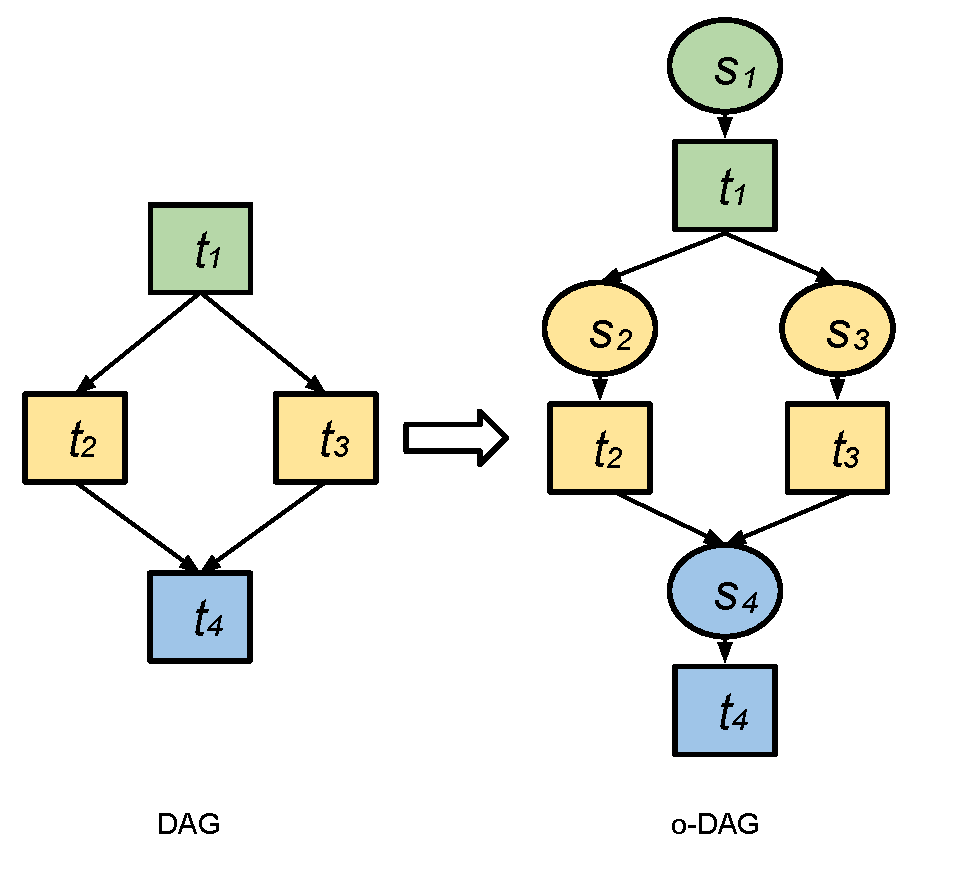
\includegraphics[width=0.7\linewidth]{figures/model/odag_color.pdf}
	\captionof{figure}{Extending DAG to o-DAG. "s" denotes a system overhead. }
	\label{fig:model_odag}
\end{figure}

Figure~\ref{fig:model_system} shows a typical workflow execution environment. The submit host prepares a workflow for execution (clustering, mapping, etc.), and worker nodes, at an execution site, execute jobs individually. The main components are introduced below:

\begin{figure}[!htb]
\centering
  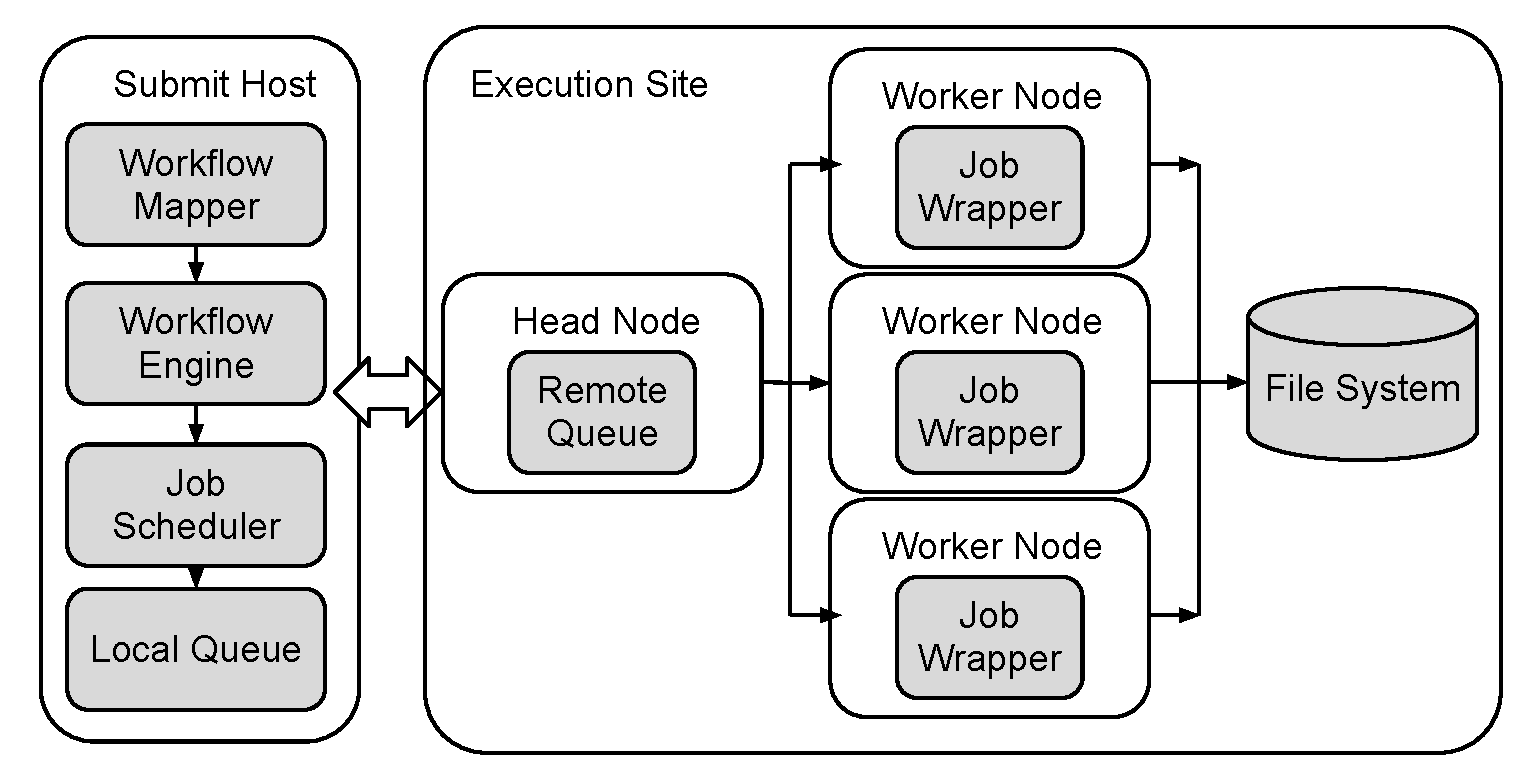
\includegraphics[width=0.95\linewidth]{figures/model/execution.pdf}
  \caption{A workflow system model.}
  \label{fig:model_system}
\end{figure}

\paragraph{Workflow Mapper} Generates an executable workflow based on an abstract workflow provided by the user or workflow composition system. It also restructures the workflow to optimize performance and adds tasks for data management and provenance information generation. In this work, the workflow mapper is used to merge small tasks together into a job such that system overheads are reduced (\textbf{task clustering}). A job is a single execution unit in the workflow execution systems and is composed of one or more tasks. 


\paragraph{Workflow Engine} Executes jobs defined by the workflow in order of their dependencies. Only jobs that have all their parent jobs completed are submitted to the Job Scheduler. The Workflow Engine relies on the resources (compute, storage, and network) defined in the executable workflow to perform computations. The elapsed time from when a job is released (all of its parents have completed successfully) to when it is submitted to the job scheduler is denoted the workflow engine delay. %The workflow engine delay is usually configured by users to assure that the entire workflow scheduling and execution system is not overloaded. 

\paragraph{Job Scheduler and Local Queue} Manage individual workflow jobs and supervise their execution on local and remote resources. The elapsed time from when a task is submitted to the job scheduler to when it starts its execution in a worker node is denoted as the queue delay. It reflects both the efficiency of the job scheduler and the resource availability. 

\paragraph{Job Wrapper} Extracts tasks from clustered jobs and executes them at the worker nodes. The clustering delay is the  elapsed time of the extraction process.

We extend the DAG model to be overhead aware (o-DAG). System overheads play an important role in workflow execution and constitute a major part of the overall runtime when tasks are poorly clustered~\cite{Chen2011}. Figure~\ref{fig:model_odag} shows how we augment a DAG to be an o-DAG with the capability to represent system overheads ($s$) such as workflow engine and queue delays. In addition, system overheads also include data transfer delay caused by staging-in and staging-out data. This classification of system overheads is based on our prior study on workflow analysis~\cite{Chen2011}. 

With an o-DAG model, we can explicitly express the process of task clustering. In this work, we address task clustering horizontally and vertically. \textbf{Horizontal Clustering} (HC) merges multiple tasks that are at the same horizontal level of the workflow, in which task horizontal level is defined as the furthest distance from the root task to this task. \textbf{Vertical Clustering} (VC) merges tasks within a pipeline of the workflow. Tasks at the same pipeline share a single-parent-single-child relationship, which means a task $t_a$ is the unique parent of a task $t_b$, which is the unique child of $t_a$. 

Figure~\ref{fig:model_hc} shows a simple example of how to perform HC, in which two tasks $t_2$ and $t_3$, without data dependency between them, are merged into a clustered job $j_1$. A job $j$ is a single execution unit composed by one or multiple task(s). Job wrappers are commonly used to execute clustered jobs, but they add an overhead denoted the clustering delay $c$. The clustering delay measures the difference between the sum of the actual task runtimes and the job runtime seen by the job scheduler. 
After horizontal clustering, $t_2$ and $t_3$ in $j_1$ can be executed in sequence or in parallel, if supported. In this work, we consider sequential executions only. Given a single resource, the overall runtime for the workflow in Figure~\ref{fig:model_hc} (left) is $runtime_l= \sum_{i=1}^{4}(s_i+t_i)$, and the overall runtime for the clustered workflow in Figure~\ref{fig:model_hc} (right) is $runtime_r=s_1+t_1+s_2+c_1+t_2+t_3+s_4+t_4$.  $runtime_l > runtime_r$ as long as $c_1 < s_3$, which is the case in many distributed systems since the clustering delay within an execution node is usually shorter than the scheduling overhead across different execution nodes. 

\begin{figure}[!htb]
\centering
 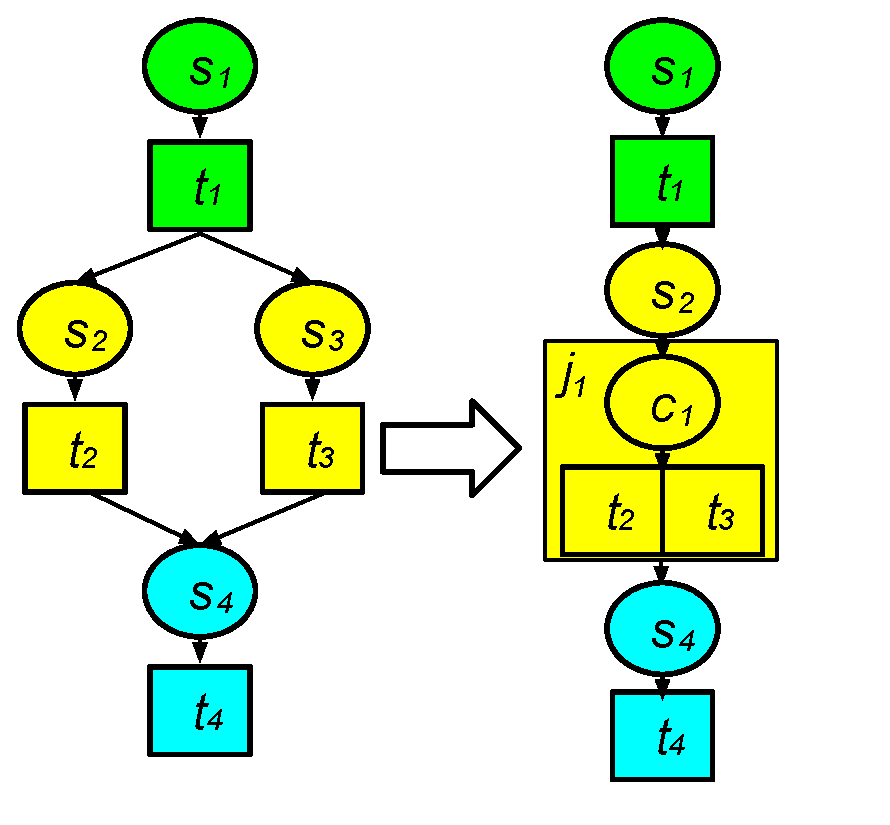
\includegraphics[width=0.55\linewidth]{figures/model/hc_color.pdf}
  \captionof{figure}{An example of horizontal clustering (color indicates the horizontal level of a task).}
  \label{fig:model_hc}
\end{figure}

Figure~\ref{fig:model_vc} illustrates an example of vertical clustering, in which tasks $t_2$, $t_4$, and $t_6$ are merged into $j_1$, while tasks $t_3$, $t_5$, and $t_7$ are merged into $j_2$. Similarly, clustering delays $c_2$ and $c_3$ are added to $j_1$ and $j_2$ respectively, but system overheads $s_4$, $s_5$, $s_6$, and $s_7$ are removed. 

\begin{figure}[!htb]
\centering
 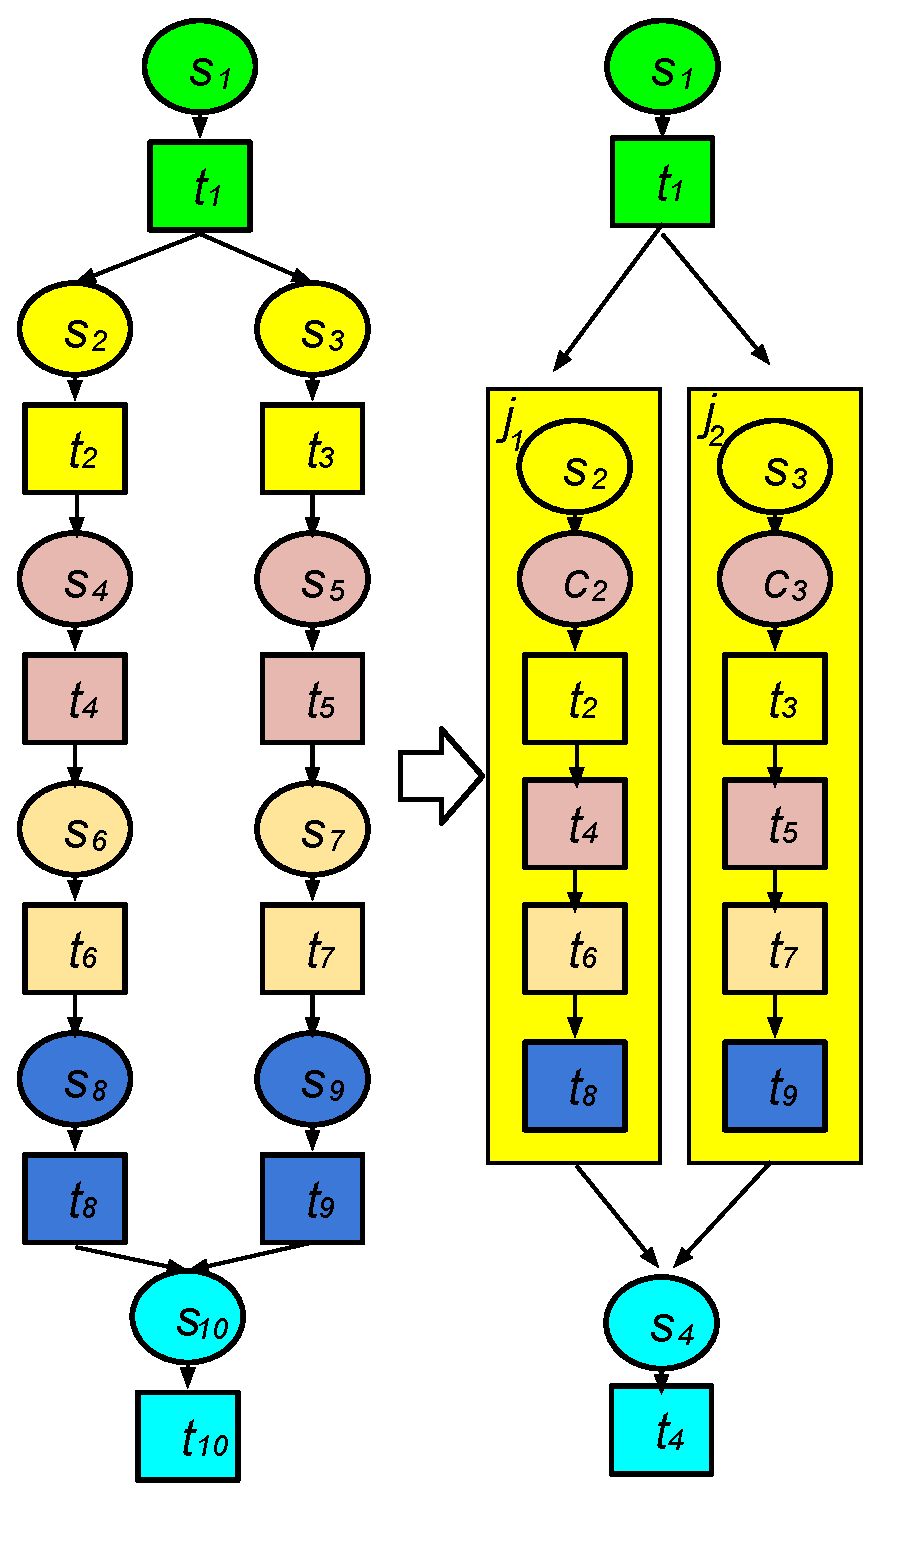
\includegraphics[width=0.6\linewidth]{figures/model/vc_color.pdf}
  \captionof{figure}{An example of vertical clustering.}
  \label{fig:model_vc}
\end{figure}

%Task clustering has been applied to many scenarios where resources are much less than tasks, which is true for many scientific workflows~\cite{Singh2008, Ying2009, Zomaya2004}, and has achieved significant improvement (i.e., 97\% as reported by ~\cite{Singh2008}) over the case without clustering. Table~\ref{tab:model_stats} shows the statistical workflow information (average task runtime etc. ) of six widely used scientific applications and their runtime information (number of nodes, average queue delay, etc.)~\cite{Chen2011}. For all of these workflows, there are a lot more tasks than available nodes and the average task runtime is shorted than system overheads. Therefore, task clustering can achieve significant improvement over no clustering. Besides the benefits of runtime improvement, task clustering also allows us to run on some federated distributed environment. For example, FutureGrid~\cite{FutureGrid} allows a user to use up to 20 VMs at a time. We will introduce the details of these workflows and distributed platforms in Session~\ref{sec:experiments}

%\begin{table*}[htbp]
%\centering
%\begin{tabular}{lrrrrrrrr}
%\hline
%Workflow & Venue & Nodes & Tasks & Workflow Engine Delay  &  Queue Delay  & Task Runtime  \\
%
%\hline
%
%SIPHT & UW Madison & 8 & 33 & 17 & 69 & 20\\ 
%Broadband & Amazon EC2 & 8 &770 & 17 &945&308\\
%Epigenomics &Amazon EC2&8& 83 &6&311&158\\
%CyberShake &Skynet&5&24142&12&188&5\\
%Montage &USC&20&10427&182&26136&523\\
%
%
%\hline
%\end{tabular}
%\caption{Overhead (in seconds) and Runtime Information }
%\label{tab:model_stats}
%\end{table*} 


\section{Overlapping Metrics}
\label{sec:profiling}

The realistic characteristics of workflows are critical to optimal workflow orchestration and profiling is an effective approach to investigate the behaviors of many complex applications. In this paper, we particularly focus on the overlapped and cumulative overheads of workflow events because this approach represents a promising trend of optimizing workflows and there is a lack of supporting analysis tools.

Workflow is typically a graph of computational activities, data transfer and system overheads as shown in our o-DAG model. Different branches of these activities may overlap with each other in the timeline and our major concern is their cumulative projection on the timeline or makespan. People have been exploring on new approaches to overlap these overheads without the necessity of reducing them. However, the challenge is how these overlapped activities contribute to the eventual makespan and how to reveal their overlapping effects in timeline from different aspects.  

%With cumulative overhead metrics, we can tell whether a workflow optimization method fully utilizes the overlap between overheads and computational activities. 

Fig.~\ref{fig:model_overhead_timeline} shows the timeline of the workflow in Fig.~\ref{fig:model_odag}. In this simple example, we are interested in questions such as: (1) whether the workflow engine delay has a good overlapping within itself? (2) wether the queue delay has a good overlapping with other types of overheads? (3) whether those 'bottleneck' overheads have overlapped with others? In the rest of this section, we will use this workflow as an example to show how we implement these metrics. 

\begin{figure*}[!htb]
	\centering
    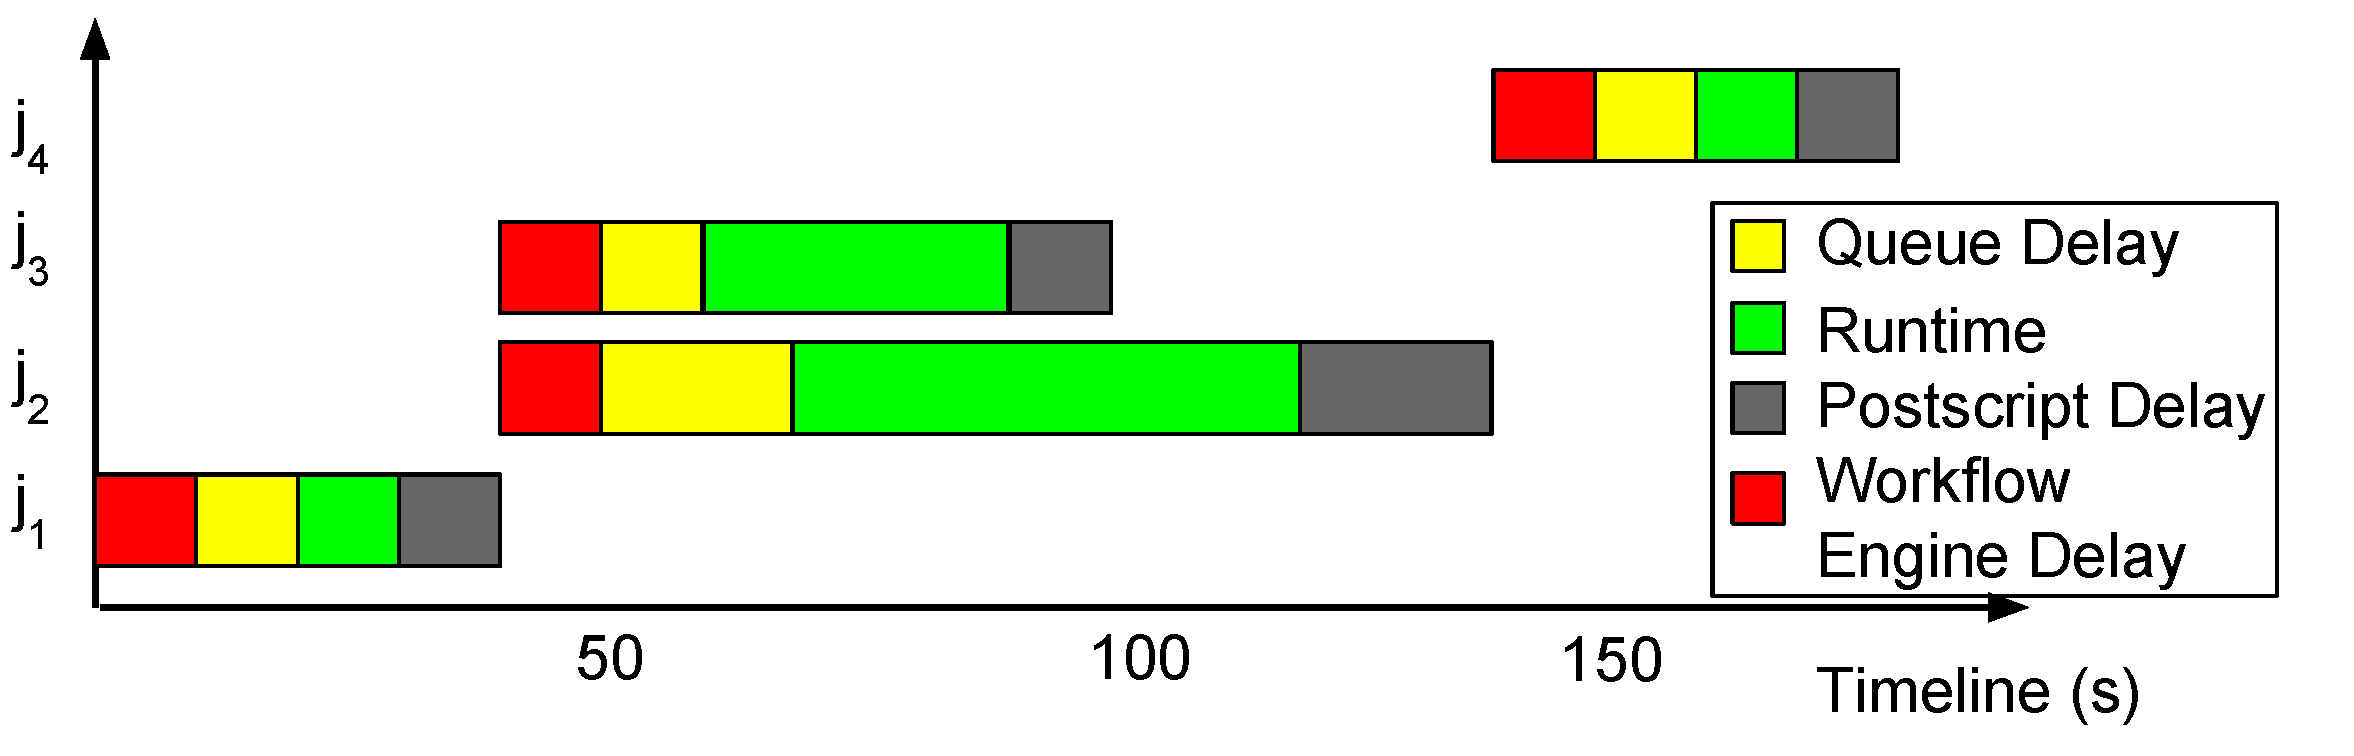
\includegraphics[width=0.7\textwidth]{figures/profiling/overhead_timeline.pdf}
    \caption{Workflow Timeline}
    \label{fig:profiling_overhead_timeline}
\end{figure*}

\begin{figure*}[!htb]
	\centering
 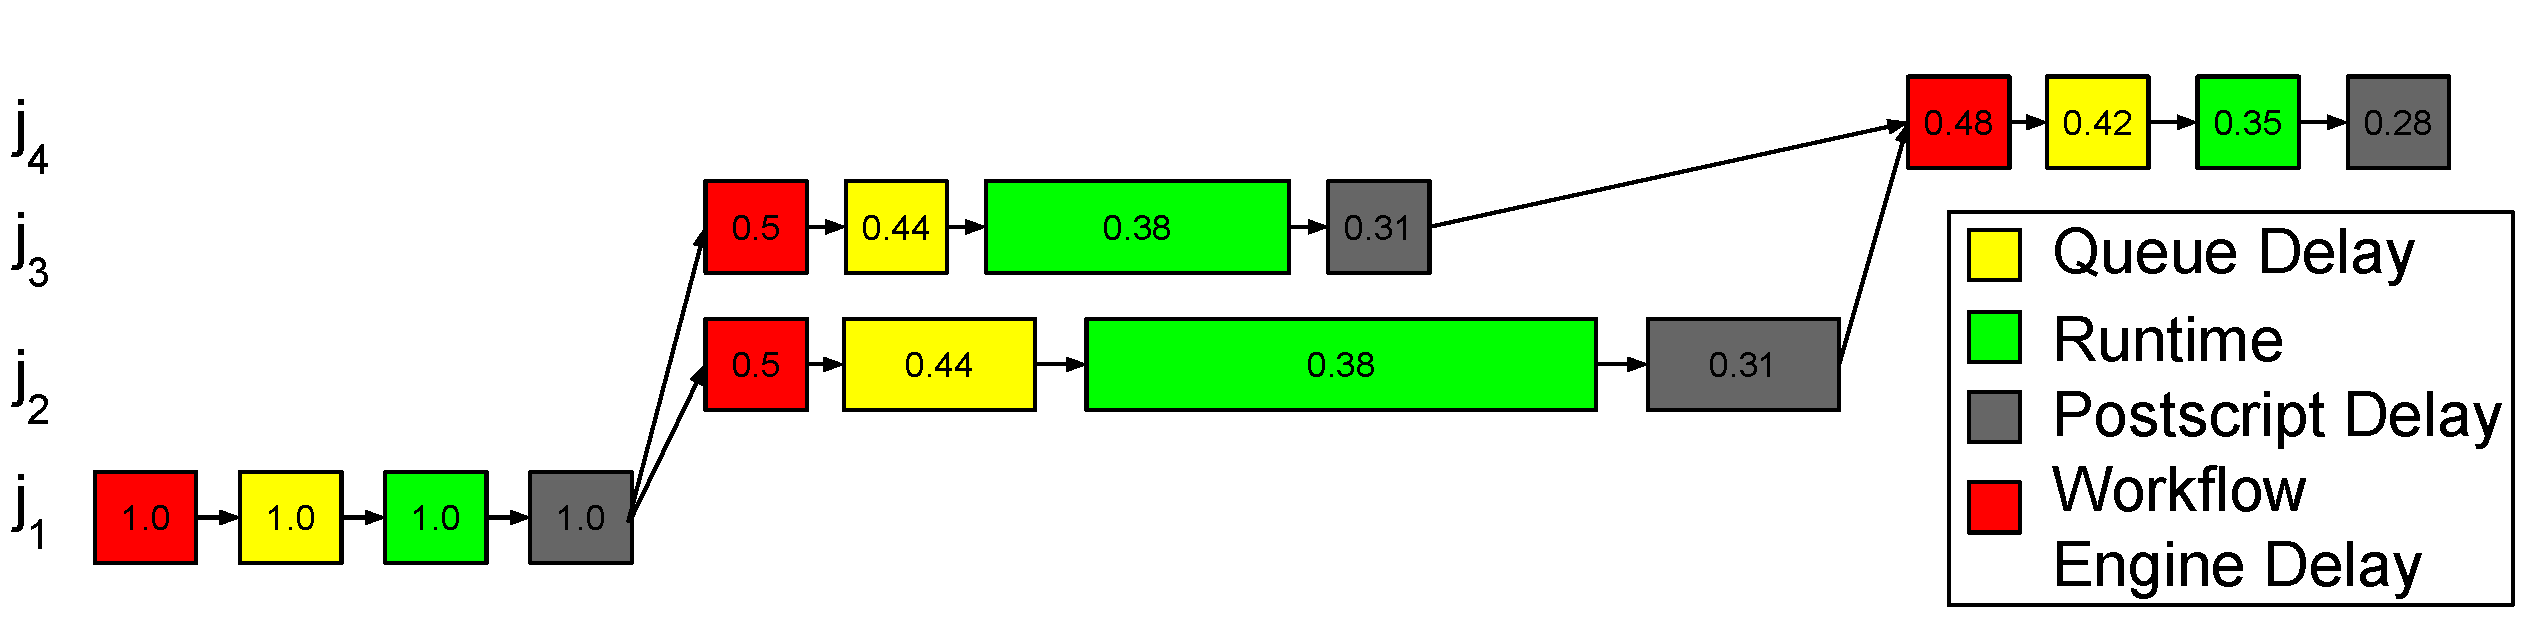
\includegraphics[width=0.8\textwidth]{figures/profiling/rr.pdf}
    \caption{Impact Factor}
    \label{fig:profiling_overhead_rr}
\end{figure*}


\subsection{Metrics to Evaluate Cumulative Overheads and Runtimes}

In this section, we propose four metrics to calculate cumulative overheads of workflows, which are $Sum$, $Projection(PJ)$, $Exclusive~Projection(EP)$ and $Impact~Factor(IF)$. $Sum$ simply adds up the overheads of all jobs without considering their overlap. $PJ$ subtracts from $Sum$ all overlaps of the same type of overhead. It is equal to the projection of all overheads to the timeline. $EP$ subtracts the overlap of all types of overheads from $PJ$. It is equal to the projection of overheads of a particular type excluding all other types of overheads to the timeline. $IF$ uses a reverse ranking algorithm to index overheads and then calculates the cumulative overhead weighted by the ranks (impact factors). The idea is brought by web page indexing algorithms such as PageRank \cite{PageRank1999}. The calculation of $Sum$, $PJ$ and $EP$ is straightforward and Fig.~\ref{fig:profiling_overhead_rr} shows how to calculate the impact factor $(IF)$ of the same workflow graph in Fig.~\ref{fig:profiling_overhead_timeline}. Both $PJ$ and $EP$ are proposed to answer Questions (1) and (2) and $IF$  answers Question (3), while $Sum$ serves as a comparison for them. 

\begin{equation} \label{eq:profiling_rr}
IF(j_u)=d+(1-d)\times\sum_{j_v\in Child(j_u)}{}\frac{IF(j_v)}{||Parent(j_v)||}
\end{equation}

Equation~\ref{eq:profiling_rr} means that the $IF$ of a node (overhead or job runtime) is determined by the $IF$ of its child nodes. $d$ is the damping factor, which controls the speed of the decrease of the $IF$. $||Parent(j_v)||$ is the number of parents that node $j_v$ has. Intuitively speaking, a node is more important if it has more children and/or its children are more important. In terms of workflows, it means an overhead has more power to control the release of other overheads and computational activities. There are two differences compared to the original PageRank:  
\begin{enumerate}
\item We use output link pointing to child nodes while PageRank uses input link from parent nodes, which is why we call it reverse ranking algorithm.
\item Since a workflow is a DAG, we do not need to calculate $IF$ iteratively. For simplicity, we assign the $IF$ of the root node to be 1. And then we calculate the $IF$ of a workflow ($G$) based on the equation below, while $\phi_{j_u}$ indicates the duration of node $j_u$.  

\begin{equation} \label{eq:profiling_sum_rr}
IF(G)=\sum_{}{}IF(j_u) \times \phi_{j_u}
\end{equation}

\end{enumerate}

$IF$ has two important features: (1) $IF$ of a node indicates the importance of this node in the whole workflow graph and its likelihood to be a bottleneck, the greater the more important; (2) $IF$ decreases from the top of the workflow to down, the speed of which is controlled by the damping factor $d$. It reflects the intuition that the overhead occurred at the beginning of the workflow execution is likely to be more important than that at the end.
By analyzing these four types of cumulative overheads, researchers have a clearer view of whether their optimization methods have overlapped the overheads of a same type (if $PJ < Sum$) or other types (if $EP < PJ$). Besides importance, $IF$ is also able to show the connectivity within the workflow, the larger the denser. 
We use a simple example workflow with four jobs to show how to calculate the overlap and cumulative overheads. Fig.~\ref{fig:profiling_overhead_timeline} shows the timeline of our example workflow. $j_1$ and $j_4$ are the parent and children of $j_2$ and $j_3$ respectively.
\begin{table*}[htb!]
\caption{Overhead and Runtime Information}
\label{tab:profiling_stats}
\centering
\begin{tabular}{lrrrrrr}
\hline
Job & Release Time &Queue Delay & Workflow Engine Delay & Runtime &Postscript Delay\\

\hline

$j_1$ & 0 & 10 & 10 & 10 & 10\\ 
$j_2$ & 40 & 10 &20 &50&20\\
$j_3$ &40&10&10&30&10\\
$j_4$ &150&10&10&10&10\\

\hline
\end{tabular}
\end{table*} 


At $t$=0,  $j_1$ is first released and once it is done at $t$=40, $j_3$ and $j_2$ are released. Finally, at $t$=140, $j_4$ is released. Table.~\ref{tab:profiling_stats} shows their overhead and runtime duration (assuming). 
For example, $PJ$ of queue delay is 40 since the queue delay of $j_2$ and $j_3$ overlaps from $t$=50 to 60. $EP$ of queue delay is 10 less than $PJ$ of queue delay since the queue delay of $j_2$ overlaps with the runtime of $j_3$ from $t$=60 to 70. 
%We show how to calculate the cumulative overheads:
 
%For $Sum$:
%$Sum(runtime)=50+30=80$. It contains the time slots of [60, 90] and [70, 120]. 
%$Sum(queue~delay)=10+20+10=40$. It contains [10, 20], [50, 70] and [50, 60]. 
%$Sum(workflow~engine~delay)=10+10+10=30$. It contains [0,10], [40, 50] and [40, 50]. 
%$Sum(postscript~delay)=10+20+10=40$. It contains [30, 40], [90, 100] and [120, 140]. 
%$Sum(data~transfer~delay)=10$. It contains [20, 30].

%For $PJ$:
%$PJ(runtime)=50+30-20=60$. It contains [60, 120].
%$PJ(queue~delay)=10+20+10-10=30$. It contains [10, 20] and [50, 70].
%$PJ(workflow~engine~delay)=10+10+10-10=20$. It contains [0, 10] and [40, 50].
%$PJ(postscript~delay)=10+20+10=40$. It contains [30, 40], [90, 100] and [120, 140].
%$PJ(data~transfer~delay)=10$. It contains [20, 30].

%For $EP$: 
%$EP(runtime)=50+30-20-10-10=40$. It contains [70, 90] and [100, 120].
%$EP(queue~delay)=10+20+10-10-10=20$. It contains [10, 20] and [50, 60]. 
%$EP(workflow~engine~delay)=10+10+10-10=20$. It contains [0, 10] and [40, 50]. 
%$EP(postscript~delay)=10+20+10-10=30$. It contains [30, 40] and  [120,140]. 
%$EP(data~transfer~delay)=10$. It contains [20, 30].

%$RR(runtime)=50\times 0.31+30\times 0.31=24.8$.
%$RR(queue~delay)=10\times 1.00+10\times 0.41+10\times 0.41=18.2$.
%$RR(workflow~engine~delay)=10\times 1.00+10\times 0.50+10\times 0.50=20$.
%$RR(postscript~delay)=10\times 1.00+10\times 0.19+20\times 0.19=15.7$.
%$RR(data~transfer~delay)=10\times 1.00=10$.

For simplicity, we do not include the data transfer delay, prescript delay and others. The overall makespan for this example workflow is 180. Table~\ref{tab:model_percentage_overhead} shows the percentage of overheads and job runtime over makespan.  

\begin{table}[h!]
\caption{Percentage of Overheads and Runtime}
\label{tab:model_percentage_overhead}
\centering
\begin{tabular}{lrrrr}
\hline
Contribution & Sum & PJ & EP &IF\\

\hline

runtime(\%) & 57.1 & 42.8 & 28.5 &17.7 \\
queue delay(\%) & 28.5 &21.4 &14.2 &13.0 \\
workflow engine delay(\%) & 21.4 &14.2& 14.2 &14.2\\
postscript delay(\%) & 28.5 & 28.5 & 21.4 & 11.2 \\
\hline
\end{tabular}
\end{table} 


In Table~\ref{tab:model_percentage_overhead}, we can conclude that the sum of $Sum$ is larger than makespan and smaller than makespan$\times$(number of resources) because it does not count the overlap at all. $PJ$ is larger than makespan since the overlap between more than two types of overheads may be counted twice or more. $EP$ is smaller than makespan since some overlap between more than two types of overheads may not be counted.  $RR$ shows how intensively these overheads and computational activities are connected to each other. 

\subsection{Experiments and Evaluations}

We applied these four metrics to a widely used workflow in our experiments. These workflows were run on distributed platforms including clouds, grids and dedicated clusters. 
On clouds, virtual machines were provisioned and then the required services (such as file transfer services) were deployed. 
We examined two clouds: Amazon EC2 \cite{AmazonEC2}  and FutureGrid \cite{FutureGrid}. Amazon EC2 is a commercial, public cloud that is been widely used in distributed computing. 
We examined the overhead distributions of a widely used astronomy workflow called Montage \cite{Berriman2004} that is used to construct large image mosaics of the sky. Montage was run on FutureGrid \cite{FutureGrid}. FutureGrid is a distributed, high-performance testbed that provides scientists with a set of computing resources to develop parallel, grid, and cloud applications. 
%Should be included in final defense
\subsection{Relationship between Overhead Metrics and Overall Performance}

In this section, we aim to investigate the relationship between the overhead metrics that we proposed and the overall performance of popular workflow restructuring techniques. Among them, task clustering \cite{Singh2008} is a technique that increases the computational granularity of tasks by merging small tasks together into a clustered job, reducing the impact of the queue wait time and also the makespan of the workflow. Data or job throttling \cite{Humphrey2008} limits the amount of parallel data transfer to avoid overloading supporting services such as data servers. Throttling is especially useful for unbalanced workflows in which one task might be idle while waiting for data to arrive. The aim of throttling is to appropriately regulate the rate of data transfers between the workflow tasks via data transfer servers by ways of restricting the data connections, data threads or data transfer jobs. Provisioning tools often deploy pilot jobs as placeholders for the execution of application jobs. Since a placeholder can allow multiple application jobs to execute during its lifetime, some job scheduling overheads can be reduced. 

\subsubsection{How Task Clustering Reduces Overheads}

\begin{table}[htb]
	\footnotesize
	\centering
	\begin{tabular}{l|rrrr}
Metric & Workflow Engine Delay  &Queue Delay& Runtime\\
		\hline
		SUM & $1.5\times 10^5$ & $1.9\times 10^7$ &  $1.5\times 10^6$ \\
		SUM/n & 54(0.16\%) & $6.8\times 10^3$(20\%)& 515(1.6\%) \\
		PJ & $3.2\times 10^3$(9.3\%) & $2.9\times 10^4$(85\%) & $3.3\times 10^4$(102\%) \\
		EP & 70(0.2\%) & 665(1.9\%) & $4.5\times 10^3$(14\%) \\
		IF & 310(0.9\%)& $1.6\times 10^4$(45\%) & $3.1\times 10^3$(9.4\%)\\
	\end{tabular}
		\caption{Metrics Without Task Clustering}
		\label{tab:profiling_no_clustering}
	\quad
	\begin{tabular}{l|rrrr}
Metric & Workflow Engine Delay  &Queue Delay& Runtime\\
		\hline
		SUM & 681(74\%) & $1.0\times 10^3$(112\%) &  $4.4\times 10^3$(475\%) \\
		SUM/n & 6.6(0.72\%) & 10(1.1\%)& 43(4.6\%) \\
		PJ & 116(13\%) & 197(21\%) & 660(72\%) \\
		EP & 72(7.8\%) & 90(9.8\%) & 420(46\%) \\
		IF & 117(13\%)& 165(18\%) & 442(48\%)\\
	\end{tabular}
		\caption{Metrics with Task Clustering}
	\label{tab:profiling_clustering}
\end{table}

In the following sections, we use a Montage workflow to show how different optimization methods improve overall performance. Many workflows are composed of thousands of fine computational granularity tasks. Task clustering is a technique that increases the computational granularity of tasks by merging small jobs together into a clustered job, reducing the impact of the queue wait time and minimizing the makespan of the workflow. Table.~\ref{tab:profiling_clustering} and Table.~\ref{tab:profiling_no_clustering} compare the overheads and runtime of the Montage workflow. $SUM/n$ indicates the average overhead or runtime per job.The percentage is calculated by the cumulative overhead ($PJ$, $EP$ or $IF$) divided by the makespan of workflows. 
In this example, we can see that $PJ$, $EJ$ and $IF$ consistently show that the portion of runtime is increased compared to overheads with task clustering. For example, the $IF$ of queue delay without clustering (45\%) is much larger than the $IF$ of runtime (9.4\%). In the case of task clustering, the $IF$ of runtime (48\%) is much larger than the $IF$ of queue delay (18\%). We can conclude that task clustering improves the runtime performance by reducing the influence of queue delay (more specifically, overlapping). The metric $SUM$ and $SUM/n$, which are usually used in other work, do not provide useful insight for us. 

\subsubsection{How Job Throttling Reduces Overheads}

\begin{table}[htb]
	\footnotesize
	\centering
	\begin{tabular}{l|rrrr}
Metric & Workflow Engine Delay  &Queue Delay& Runtime\\
		\hline
		SUM & $9.2\times 10^4$ & $1.7\times 10^5$ &  $9.2\times 10^3$ \\
		SUM/n & 32(2.6\%) & 60(4.8\%)& 3.2(0.3\%) \\
		PJ & 558(44.6\%) & 873(70\%) & 990(79\%) \\
		EP & 84(6.7\%) & 90(7.2\%) & 190(15.2\%) \\
		IF & 162(13\%)& 331(27\%) & 205(16.4\%)\\
	\end{tabular}
		\caption{Metrics with Throttling ($p$=24)}
		\label{tab:profiling_throttling_24}
	\quad
	\begin{tabular}{l|rrrr}
Metric & Workflow Engine Delay  &Queue Delay& Runtime\\
		\hline
		SUM & $7.4\times 10^4$ & $1.6\times 10^5$ &  $6.5\times 10^3$ \\
		SUM/n & 25.9(2.2\%) & 57(4.9\%)& 2.3(0.2\%) \\
		PJ & 561(47.5\%) & 856(72.5\%) & 928(78.6\%) \\
		EP & 77(6.5\%) & 75(6.4\%) & 140(11.9\%) \\
		IF & 153(13\%)& 307(26\%) & 187(15.8\%)\\
	\end{tabular}
		\caption{Metrics with Throttling ($p$=16)}
		\label{tab:profiling_throttling_16}
	\quad
	\begin{tabular}{l|rrrr}
Metric & Workflow Engine Delay  &Queue Delay& Runtime\\
		\hline
		SUM & $9.2\times 10^4$ & $1.7\times 10^5$ &  $9.2\times 10^3$ \\
		SUM/n & 32(2.5\%) & 59(4.7\%)& 3.2(0.3\%) \\
		PJ & 520(41\%) & 896(71\%) & 1073(85\%) \\
		EP & 75(5.9\%) & 70(5.5\%) & 185(14.6\%) \\
		IF & 142(11.2\%)& 326(25.7\%) & 223(17.6\%)\\
	\end{tabular}
		\caption{Metrics with Throttling ($p$=12)}
	\label{tab:profiling_throttling_12}
\end{table}


Data or job throttling limits the amount of parallel data transfer to avoid overloading supporting services such as data servers. Throttling is especially useful for unbalanced workflows in which one task might be idle while waiting for data to arrive. The aim of throttling is to appropriately regulate the rate of data transfers between the workflow tasks via data transfer servers by ways of restricting the data connections, data threads or data transfer jobs. Especially on cloud platforms, I/O requests need to go through more layers than a physical cluster; and thereby workflows may suffer a higher overhead from data servers.

In our experiments, the data transfer service is deployed on a virtual machine that is similar to a worker node.  In this section, we evaluate a simple static throttling strategy where the Condor scheduler limits the number of concurrent jobs to be run and thereby restricts the number of parallel I/O requests. There are 32 resources available and we evaluate the cases with throttling parameters ($p$, the maximum jobs in queue) that are equal to 24, 16 and 12 respectively. In the case of $p$=24, the resources are better utilized but the data server is heavily loaded. In the case of $p$=12, the resources are under-utilized even though the data server has more capabilities. Table.~\ref{tab:profiling_throttling_24, tab:profiling_throttling_16, tab:profiling_throttling_12} show the contribution of workflow overheads and runtime. With limited throttling (reducing threshold from 24 to 16), the data transfer requests are distributed in the timeline more evenly and, as a result, their overhead is reduced. However, with over throttling (reducing threshold from 16 to 12), resources are not fully utilized and thus the makespan is increased. In this experiment, $PJ$, $EP$ and $IF$ reflect the variation trend of overheads and makespan better than $SUM$ and $SUM/n$. 

%\textbf{How Pre-staging Reduces Overheads}

%Scientific workflows often consume and produce a large amount of data during execution. Data pre-staging [14] transfers input data before the computational activities are started or even before the workflow is mapped onto resources. Data placement policies distribute data in advance by placing data sets where they may be requested or by replicating data sets to improve runtime performance. In our experiments, because data is already pre-staged, the implementation of the stage-in job is to create a soft link to the data from the workflow’s working directory, making it available to the workflow jobs. Table 4.4 and Fig. 4.9 show the cumulative overheads and runtime of the Montage workflows running with and without pre-staging. Looking at the rows for $PJ$ in Table 4.4, we can conclude that pre-staging improves the overall runtime by reducing the data transfer delay. For the case without pre-staging the $EP$ for data transfer delay is zero because it overlaps with the workflow engine delay of another job. Therefore, in this experiment, $PJ$ reflects the variation trend of the makespan more consistently. 

\subsubsection{How Provisioning Reduces Overheads}

\begin{table}[htb]
	\footnotesize
	\centering
	\begin{tabular}{l|rrrr}
Metric & Workflow Engine Delay  &Queue Delay& Runtime\\
		\hline
		SUM & $1.5\times 10^5$ & $1.9\times 10^7$ &  $1.5\times 10^6$ \\
		SUM/n & 54(0.16\%) & $6.8\times 10^3$(20\%)& 515(1.6\%) \\
		PJ & $3.2\times 10^3$(9.3\%) & $2.9\times 10^4$(85\%) & $3.3\times 10^4$(102\%) \\
		EP & 70(0.2\%) & 665(1.9\%) & $4.5\times 10^3$(14\%) \\
		IF & 310(0.9\%)& $1.6\times 10^4$(45\%) & $3.1\times 10^3$(9.4\%)\\
	\end{tabular}
		\caption{Metrics Without Resource Provisioning}
			\label{tab:profiling_no_provisioning}
	\quad
	\begin{tabular}{l|rrrr}
Metric & Workflow Engine Delay  &Queue Delay& Runtime\\
		\hline
		SUM & $8.1\times 10^4$ & $5.0\times 10^5$ &  $3.1\times 10^4$ \\
		SUM/n & 28(0.9\%) & 173(5.5\%)& 11(0.4\%) \\
		PJ & $1.0\times 10^3$(32\%) & $2.3\times 10^3$(74\%) & $3.0\times 10^3$(94\%) \\
		EP & 73(2.3\%) & 50(1.6\%) & 588(19\%) \\
		IF & 174(5.5\%)& 840(27\%) & 683(22\%)\\
	\end{tabular}
		\caption{Metrics with Resource Provisioning}
	\label{tab:profiling_provisioning}
\end{table}


Many of the scientific applications presented here consist of a large number of short-duration tasks whose runtimes are greatly influenced by overheads present in distributed environments. Most of these environments have an execution mode based on batch scheduling where jobs are held in a queue until resources become available to execute them. Such a best-effort model normally imposes heavy overheads in scheduling and queuing. For example, Condor-G~\cite{Frey2002} uses Globus GRAM~\cite{Foster1997} to submit jobs to remote clusters. The Globus Toolkit normally has a significant overhead compared to running Condor directly as an intra domain resource and job management system. Provisioning tools often deploy pilot jobs as placeholders for the execution of application jobs. Since a placeholder can allow multiple application jobs to execute during its lifetime, some job scheduling overheads can be reduced. In our experiments, we compared the performance of Condor-G (without provisioning) and Corral (with provisioning). 

Table.~\ref{tab:profiling_no_provisioning} and Table.~\ref{tab:profiling_provisioning} show the contribution of workflow overheads and runtime. The percentage is calculated by the cumulative overhead ($PJ$, $EP$, or $IF$) divided by the makespan of workflows. Comparing $PJ$, $EP$ and $IF$, we can conclude that the overheads with provisioning have been reduced significantly. The reason is that the local scheduler has direct control over the resources without going through Globus. 



\section{Balanced Clustering}
\label{sec:imbalance}

Task clustering has been widely used to address the low performance of very short running tasks on platforms where the system overhead is high, such as distributed computing infrastructures. However, up to now, techniques do not consider the load balance problem. In particular, merging tasks within a workflow level without considering the runtime variance may cause load imbalance (Runtime Imbalance), or merging tasks without considering their data dependencies may lead the system to data locality problems (Dependency Imbalance). In this section, we introduce metrics that quantitatively capture workflow characteristics to measure runtime and dependence imbalances. We then present methods to handle the load balance problem.


\subsection{Imbalance metrics}

\textbf{Runtime Imbalance} describes the difference of the task/job runtime of a group of tasks/jobs. In this work, we denote the \textbf{Horizontal Runtime Variance} ($HRV$) as the ratio of the standard deviation in task runtime to the average runtime of tasks/jobs at the same horizontal level of a workflow. At the same horizontal level, the job with the longest runtime often controls the release of the next level jobs. A high $HRV$ value means that the release of next level jobs has been delayed. Therefore, to improve runtime performance, it is meaningful to reduce the standard deviation of job runtime. Figure~\ref{fig:imbalance_rv} shows an example of four independent tasks $t_1$, $t_2$, $t_3$ and $t_4$ where the task runtime of $t_1$ and $t_2$ is 10 seconds, and the task runtime of $t_3$ and $t_4$ is 30 seconds. In the Horizontal Clustering (HC) approach, a possible clustering result could be merging $t_1$ and $t_2$ into a clustered job, and $t_3$ and $t_4$ into another. This approach results in imbalanced runtime, i.e., $HRV > 0$ (Figure~\ref{fig:imbalance_rv}-top). In contrast, a balanced clustering strategy should try its best to evenly distribute task runtime among jobs as shown in Figure~\ref{fig:imbalance_rv} (bottom). A smaller \emph{HRV} means that the runtime of tasks within a horizontal level is more evenly distributed and therefore it is less necessary to balance the runtime distribution. However, runtime variance is not able to describe how regular is the structure of the dependencies between tasks.

\begin{figure}[htb]
	\centering
	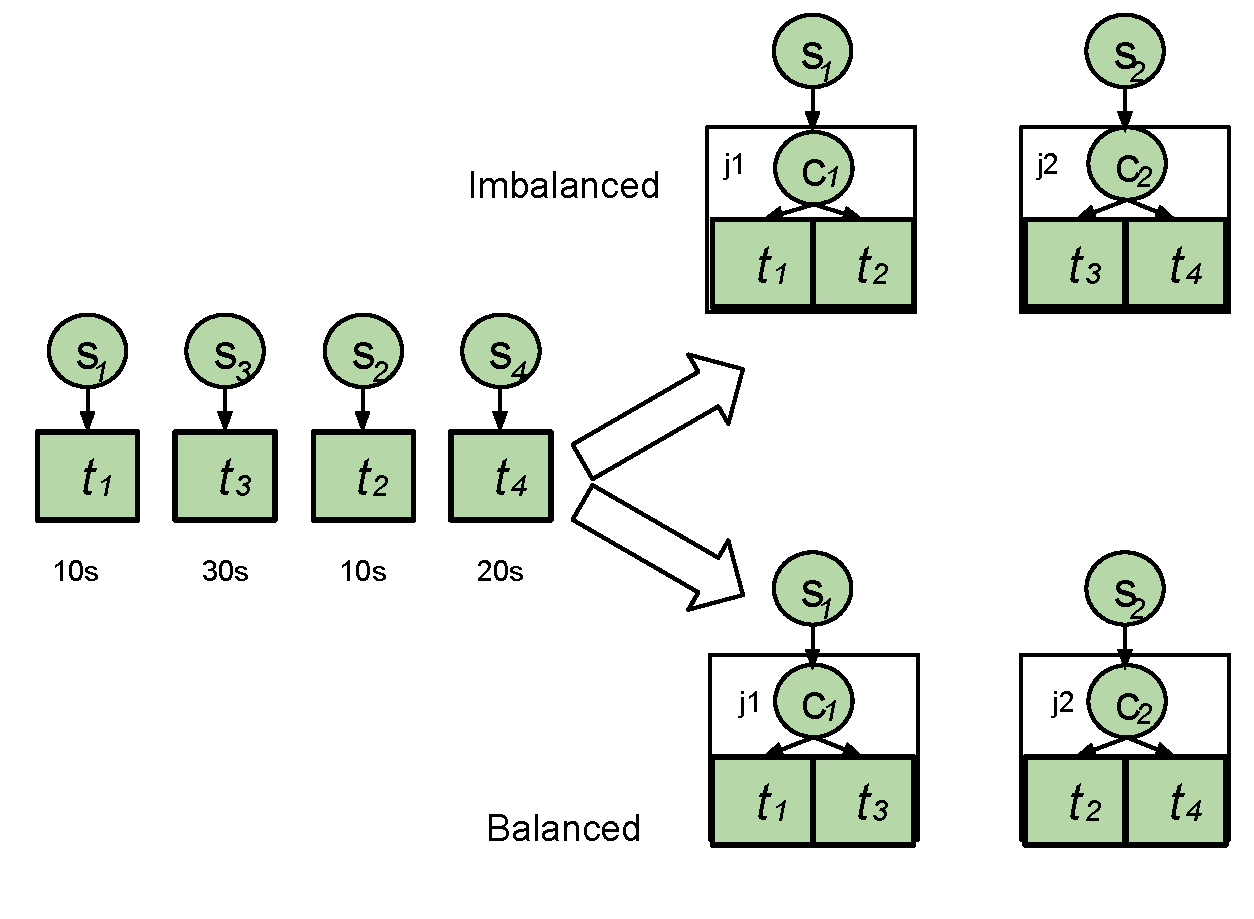
\includegraphics[width=0.95\linewidth]{figures/imbalance/runtime_variance.pdf}
	\captionof{figure}{An example of Horizontal Runtime Variance.}
	\label{fig:imbalance_rv}
\end{figure}


\textbf{Dependency Imbalance} means that the task clustering at one horizontal level forces the tasks at the next level (or even subsequent levels) to have severe data locality problems and thus loss of parallelism. For example, in Figure~\ref{fig:imbalance_dv}, we show a two-level workflow composed of four tasks in the first level and two in the second. Merging $t_1$ with $t_3$ and $t_2$ with $t_4$ (imbalanced workflow in Figure~\ref{fig:imbalance_dv}) forces $t_5$ and $t_6$ to transfer files from two locations and wait for the completion of $t_1$, $t_2$, $t_3$, and $t_4$.  A balanced clustering strategy groups tasks that have the maximum number of child tasks in common. Thus, $t_5$ can start to execute as soon as $t_1$ and $t_2$ are completed, and so can $t_6$. To measure and quantitatively demonstrate the Dependency Imbalance of a workflow, we propose two  metrics: ($i$) Impact Factor Variance, and ($ii$) Distance Variance. 

\begin{figure}[htb]
	\centering
	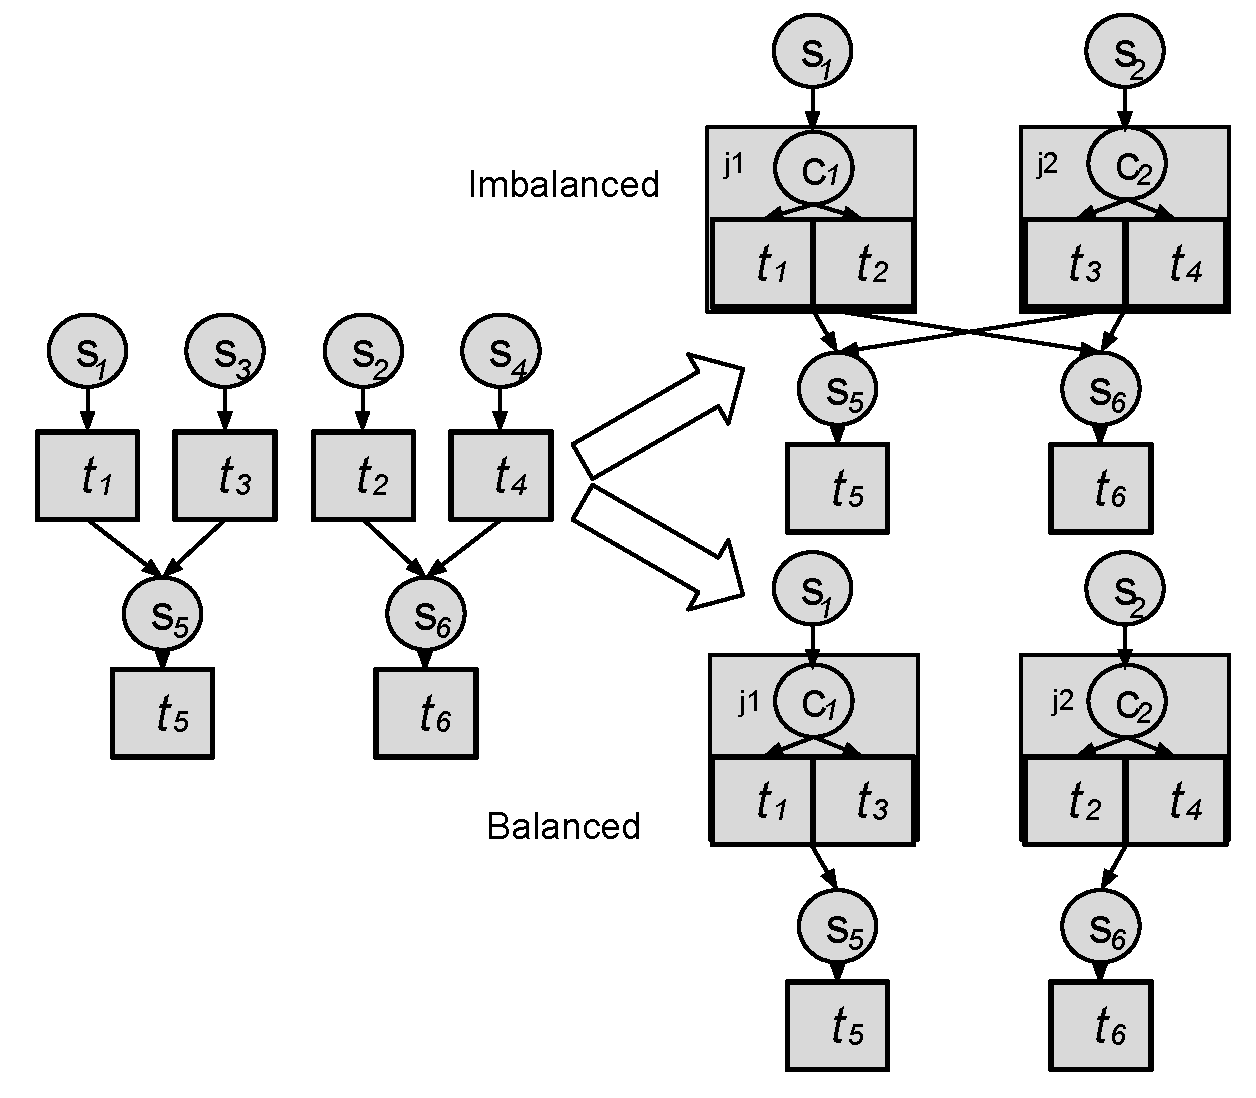
\includegraphics[width=0.95\linewidth]{figures/imbalance/dv.pdf}
	\captionof{figure}{An example of Dependency Imbalance.}
	\label{fig:imbalance_dv}
\end{figure}

We define the \textbf{Impact Factor Variance} ($IFV$) of tasks as the standard deviation of their impact factors. The Impact Factor aims at capturing the similarity of tasks/jobs in a graph by measuring their relative impact factor or importance to the entire graph. Tasks with similar impact factors are merged together, so that the workflow structure tends to be more `even' or `regular'. The \textbf{Impact Factor} ($IF$) of a task $t_u$ is defined as follows:

\begin{equation}
\label{eq:imbalance_impact_factor}
	IF(t_u)=\sum_{t_v\in Child(t_u)}^{}\frac{IF(t_v)}{||Parent(t_v)||}
\end{equation}
where $Child(t_u)$ denotes the set of child tasks of $t_u$, and $||Parent(t_v)||$ the number of parent tasks of $t_v$. For simplicity, we assume the $IF$ of a workflow exit task (e.g. $t_5$ in Figure~\ref{fig:imbalance_dv}) as 1.0. For instance, consider the two workflows presented in Figure~\ref{fig:imbalance_hifv}. $IF$ for $t_1$, $t_2$, $t_3$, and $t_4$ are computed as follows:

\begin{eqnarray}
	\displaystyle  
	&IF(t_7 )=1.0, IF(t_6 )=IF(t_5 )=IF(t_7 )/2=0.5\nonumber  \\
	&IF(t_1 )=IF(t_2 )=IF(t_5 )/2=0.25\nonumber \\
	&IF(t_3 )=IF(t_4 )=IF(t_6 )/2=0.25\nonumber 
\end{eqnarray}
Thus, IFV($t_1$, $t_2$, $t_3$, $t_4$) = 0. In contrast, $IF$ for $t_{1'}$, $t_{2'}$, $t_{3'}$, and $t_{4'}$ are:

\begin{eqnarray}
	\displaystyle  
	&IF(t_{7'})=1.0, IF(t_{6'})=IF(t_{5'})=IF(t_{1'})=IF(t_{7'})/2=0.5\nonumber \\
	&IF(t_{2'})=IF(t_{3'})=IF(t_{4'})=IF(t_{6'})/3=0.17 \nonumber
\end{eqnarray}
Therefore, the $IFV$ value for {$t_{1'}$, $t_{2'}$, $t_{3'}$, $t_{4'}$} is 0.17, which means it is less regular than the workflow in Figure~\ref{fig:imbalance_hifv} (left). In this work, we use \textbf{HIFV} (Horizontal IFV) to indicate the $IFV$ of tasks at the same horizontal level. The time complexity of calculating all the $IF$ of a workflow with $n$ tasks is $O(n)$.  

\begin{figure}[htb]
	\centering
	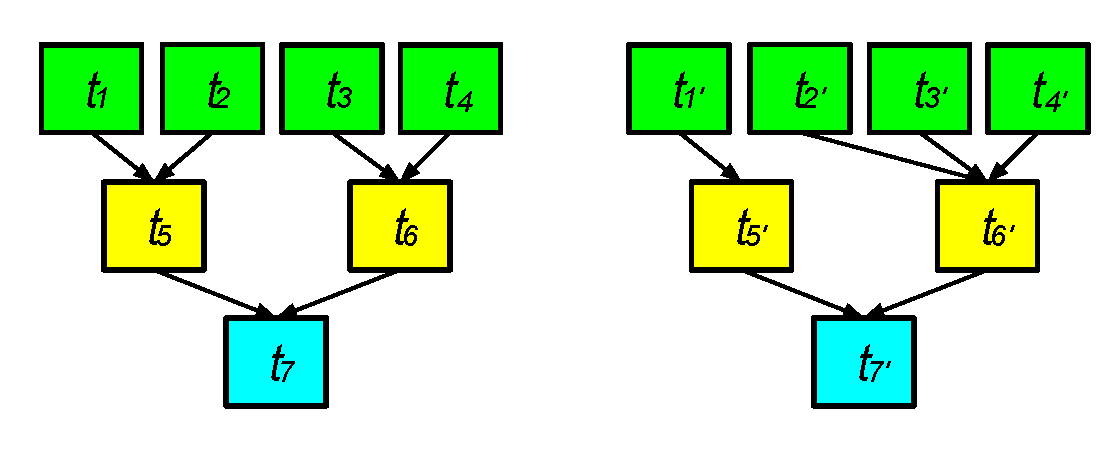
\includegraphics[width=0.85\linewidth]{figures/imbalance/dependency.pdf}
	\captionof{figure}{Example of workflows with different data dependencies (For better visualization, we do not show system overheads in the rest of the paper).}
	\label{fig:imbalance_hifv}
\end{figure}

\textbf{Distance Variance} ($DV$) describes how `close' tasks are to each other. The distance between two tasks/jobs is defined as the cumulative length of the path to their closest common successor. If they do not have a common successor, the distance is set to infinity. For a group of $n$ tasks/jobs, the distance between them is represented by a $n \times n$ matrix $D$, where an element $D(u,v)$ denotes the distance between a pair of tasks/jobs $u$ and $v$. For any workflow structure, $D(u,v)=D(v,u)$ and $D(u,u)=0$, thus we ignore the cases when $u \geq v$. Distance Variance is then defined as the standard deviation of all the elements $D(u,v)$ for $u<v$. The time complexity of calculating all the $D$ of a workflow with $n$ tasks is $O(n^2)$. 

Similarly, $HDV$ indicates the $DV$ of a group of tasks/jobs at the same horizontal level. For example, Table~\ref{tab:imblance_metric} shows the distance matrices of tasks from the first level for both workflows of Figure~\ref{fig:imbalance_hifv} ($D_1$ for the workflow in the left, and $D_2$ for the workflow in the right). $HDV$ for $t_1, t_2, t_3$, and $t_4$ is 1.03, and for $t_{1'}, t_{2'}, t_{3'}$, and $t_{4'}$ is 1.10. In terms of distance variance, $D_1$ is more `even' than $D_2$. A smaller $HDV$ means the tasks at the same horizontal level are more equally `distant' from each other and thus the workflow structure tends to be more `even' and `regular'. 

\begin{table}[htb]
	\footnotesize
	\centering
	\begin{tabular}{l|rrrr}
		$D_1$ & $t_1$ & $t_2$ & $t_3$ &$t_4$\\
		\hline
		$t_1$ & 0 & 2 & 4 & 4 \\
		$t_2$ & 2 & 0 & 4 & 4 \\
		$t_3$ & 4 & 4 & 0 & 2\\
		$t_4$ & 4 & 4 & 2 & 0 \\
	\end{tabular}
	\quad
	\begin{tabular}{l|rrrr}
		$D_2$ & $t_1'$ & $t_2'$ & $t_3'$ &$t_4'$\\
		\hline
		$t_1'$ & 0 & 4 & 4 & 4 \\
		$t_2'$ & 4 & 0 & 2 & 2 \\
		$t_3'$ & 4 & 2 & 0 & 2\\
		$t_4'$ & 4 & 2 & 2 & 0 \\
	\end{tabular}
	\caption{Distance matrices of tasks from the first level of workflows in Figure~\ref{fig:imbalance_hifv}.}
	\label{tab:imblance_metric}
\end{table}

In conclusion, runtime variance and dependency variance offer a quantitative and comparable tool to measure and evaluate the internal structure of a workflow. 



\subsection{Balanced clustering methods}
\label{sec:methods}
In this subsection, we introduce our balanced clustering methods used to improve the runtime and dependency balances in task clustering. We first introduce the basic runtime-based clustering method, and then two other balancing methods that address the dependency imbalance problem. %We use the metrics presented in the previous subsection to evaluate a given workflow to decide which balancing method(s) is(are) more appropriate. 

%Algorithm~\ref{alg:imbalance_algo} shows the pseudocode of our balanced clustering algorithm that uses a combination of these balancing methods and metrics.  The maximum number of clustered jobs (size of $CL$) is equal to the number of available resources multiplied by a \emph{clustering factor}. 

%\begin{algorithm}[htb]
%	\caption{ Balanced Clustering algorithm}
%	\footnotesize
%	\label{alg:imbalance_algo}
%	\begin{algorithmic}[1]
%		\Require $W$: workflow; $CL$: list of clustered jobs; $C$: the required size of $CL$; 
%		\Ensure The job runtime of $CL$ are as even as possible
%		\Procedure{Clustering}{$W,D,C$}
%			\State Sort $W$ in decreasing order of the size of each level
%			\For{$level < $the depth of $W$}
%				\State $TL\gets $\ \Call{GetTasksAtLevel}{$w,level$} \Comment{Partition $W$ based on depth}
%				\State $CL\gets$  \ \Call{Merge}{$TL,C$} \Comment{Form a list of clustered jobs}
%				\State $W \gets W - TL + CL$  \Comment{Merge dependencies as well} 
%			\EndFor
%		\EndProcedure
%		\Procedure{Merge}{$TL, C$}
%			\State Sort $TL$ in decreasing order of task runtime
%			\For{$t\ in\ TL$}
%				\State $J \gets $\ \Call{GetCandidateJob}{$CL, t$} \Comment{Get a candidate task}
%				\State  $J \gets J\ +\ t$ \Comment{Merge it with the clustered job}
%			\EndFor
%			\State \textbf{return} $CL$
%		\EndProcedure
%		\Procedure{GetCandidateJob}{$CL, t$}
%			\State Selects a job based on balanced clustering methods
%		\EndProcedure
%	\end{algorithmic}
%\end{algorithm}

%We examine tasks in a level-by-level approach starting from the level with the largest width (number of tasks at the same level, \texttt{line 2}). The intuition behind this breadth favored approach is that we believe it should improve the performance most. Then, we determine which type of imbalance problem a workflow experiences based on the balanced clustering metrics presented previously ($HRV$, $HIFV$, and $HDV$), and accordingly, we select a combination of balancing methods. \textsc{GetCandidateJob} selects a job (\texttt{line 12}) from a list of potential candidate jobs ($CL$) to be merged with the targeting task ($t$). Below we introduce the three balancing methods proposed in this work.


\begin{algorithm}[!htb]
	\footnotesize
	\caption{Horizontal Runtime Balancing algorithm.}
	\label{alg:imbalance_hrb}
	\begin{algorithmic}[1]
		\Require $W$: workflow; $C$: number of tasks per jobs; $R$: number of jobs per horizontal level
		\Procedure{Clustering}{$W,C$}
			\For{$level < depth(W)$}
				\State $TL\gets $\ \Call{GetTasksAtLevel}{$W,level$} \Comment{Partition $W$ based on depth}
				\State $CL\gets$  \ \Call{Merge}{$TL,C, R$} \Comment{Returns a list of clustered jobs}
				\State $W \gets W - TL + CL$  \Comment{Merge dependencies as well} 
			\EndFor
		\EndProcedure
		\Procedure{Merge}{$TL, C, R$}
			\For{$i<R$}
			\State $J_i\gets$\{\}\Comment{An empty job}
			\EndFor
			\State $CL\gets$\{\}\Comment{An empty list of clustered jobs}
			\State Sort $TL$ in descending of runtime
			\ForAll{$t$ in $TL$}
				\State $J\gets$ the job with shortest runtime and less than $C$ tasks  
				\State $J$.add ($t$) \Comment{Adds the task to the shortest job}
				
			\EndFor
			\For{$i<R$}
			\State  $CL$.add( $J_i$)
			\EndFor
			\State \textbf{return} $CL$
		\EndProcedure
	\end{algorithmic}
\end{algorithm}



\textbf{Horizontal Runtime Balancing} (HRB) aims to evenly distribute task runtime among clustered jobs. Tasks with the longest runtime are added to the job with the shortest runtime. Algorithm~\ref{alg:imbalance_hrb} shows the pseudo codes of HRB. This greedy method is used to address the load balance problem caused by runtime variance at the same horizontal level. Figure~\ref{fig:imbalance_hrb} shows an example of HRB where tasks in the first level have different runtimes and should be grouped into two jobs. HRB sorts tasks in decreasing order of runtime, and then adds the task with the highest runtime to the group with the shortest aggregated runtime. Thus, $t_1$ and $t_3$, as well as $t_2$ and $t_4$ are merged together.
For simplicity, system overheads are not displayed.


\begin{algorithm}[!htb]
	\footnotesize
	\caption{Horizontal Impact Factor Balancing algorithm.}
	\label{alg:imbalance_hifb}
	\begin{algorithmic}[1]
		\Require $W$: workflow; $C$: number of tasks per jobs; $R$: number of jobs per horizontal level
		\Procedure{Clustering}{$W,C$}
			\For{$level < depth(W)$}
				\State $TL\gets $\ \Call{GetTasksAtLevel}{$W,level$} \Comment{Partition $W$ based on depth}
				\State $CL\gets$  \ \Call{Merge}{$TL,C, R$} \Comment{Returns a list of clustered jobs}
				\State $W \gets W - TL + CL$  \Comment{Merge dependencies as well} 
			\EndFor
		\EndProcedure
		\Procedure{Merge}{$TL, C, R$}
			\For{$i<R$}
			\State $J_i\gets$\{\}\Comment{An empty job}
			\EndFor
			\State $CL\gets$\{\}\Comment{An empty list of clustered jobs}
			\State Sort $TL$ in descending of runtime
			\ForAll{$t$ in $TL$}
				\State $L\gets$ Sort all $J_i$ with the similarity of impact factors with $t$
				\State $J\gets$ the job with shortest runtime and less than $C$ tasks in $L$
				\State $J$.add ($t$) 
				
			\EndFor
			\For{$i<R$}
			\State  $CL$.add( $J_i$)
			\EndFor
			\State \textbf{return} $CL$
		\EndProcedure
	\end{algorithmic}
\end{algorithm}


\begin{algorithm}[!htb]
	\footnotesize
	\caption{Horizontal Distance Balancing algorithm.}
	\label{alg:imbalance_hdb}
	\begin{algorithmic}[1]
		\Require $W$: workflow; $C$: number of tasks per jobs; $R$: number of jobs per horizontal level
		\Procedure{Clustering}{$W,C$}
			\For{$level < depth(W)$}
				\State $TL\gets $\ \Call{GetTasksAtLevel}{$W,level$} \Comment{Partition $W$ based on depth}
				\State $CL\gets$  \ \Call{Merge}{$TL,C, R$} \Comment{Returns a list of clustered jobs}
				\State $W \gets W - TL + CL$  \Comment{Merge dependencies as well} 
			\EndFor
		\EndProcedure
		\Procedure{Merge}{$TL, C, R$}
			\For{$i<R$}
			\State $J_i\gets$\{\}\Comment{An empty job}
			\EndFor
			\State $CL\gets$\{\}\Comment{An empty list of clustered jobs}
			\State Sort $TL$ in descending of runtime
			\ForAll{$t$ in $TL$}
				\State $L\gets$ Sort all $J_i$ with the closest distance with $t$
				\State $J\gets$ the job with shortest runtime and less than $C$ tasks in $L$
				\State $J$.add ($t$) 
				
			\EndFor
			\For{$i<R$}
			\State  $CL$.add( $J_i$)
			\EndFor
			\State \textbf{return} $CL$
		\EndProcedure
	\end{algorithmic}
\end{algorithm}


%how HRB works in an example of four jobs with different job runtime (assuming the height of a job is its runtime). For the given task ($t_0$), HRB sorts the potential jobs ($j_1$, $j_2$, $j_3$, and $j_4$) based on their runtime and selects the shortest job (in this case $j_1$ or $j_2$). 

\begin{figure}[htb]
	\centering
	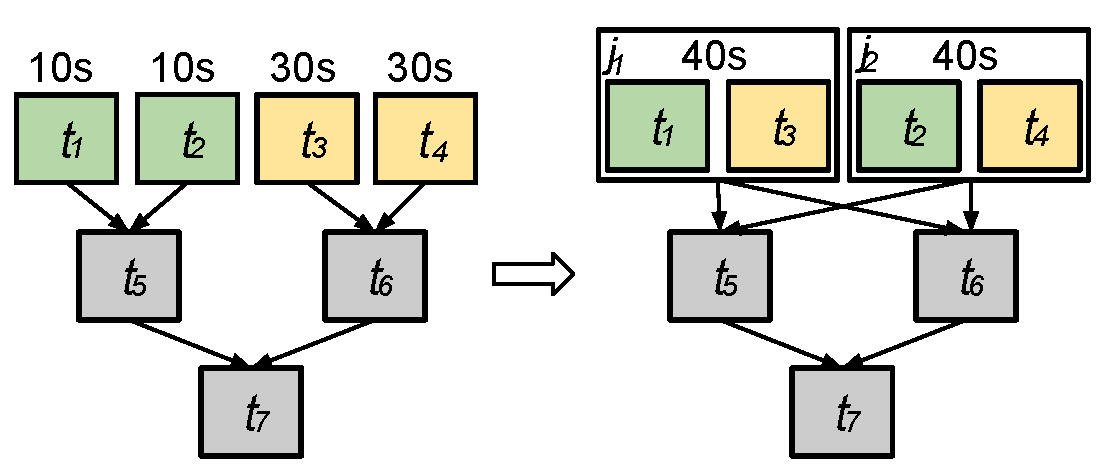
\includegraphics[width=0.85\linewidth]{figures/imbalance/hrb.pdf}
	\caption{An example of the HRB (Horizontal Runtime Balancing) method. By solely addressing runtime variance, data locality problems may arise.}
	\label{fig:imbalance_hrb}
\end{figure}

However, HRB may cause a dependency imbalance problem since the clustering does not take data dependency into consideration. To address this problem, we propose the \textbf{Horizontal Impact Factor Balancing} (HIFB) and the \textbf{Horizontal Distance Balancing} (HDB) methods. 

In HRB, candidate jobs within a workflow level are sorted by their runtime, while in HIFB jobs are first sorted based on their similarity of $IF$, then on runtime. 
Algorithm~\ref{alg:imbalance_hifb} shows the pseudo codes of HIFB. 
For example, in Figure~\ref{fig:imbalance_hifb}, $t_1$ and $t_2$ have $IF = 0.25$, while $t_3$, $t_4$, and $t_5$ have $IF = 0.16$. HIFB selects a list of candidate jobs with the same IF value, and then HRB is performed to select the shortest job. Thus, HIFB merges $t_1$ and $t_2$ together, as well as $t_3$ and $t_4$.

\begin{figure}[htb]
	\centering
	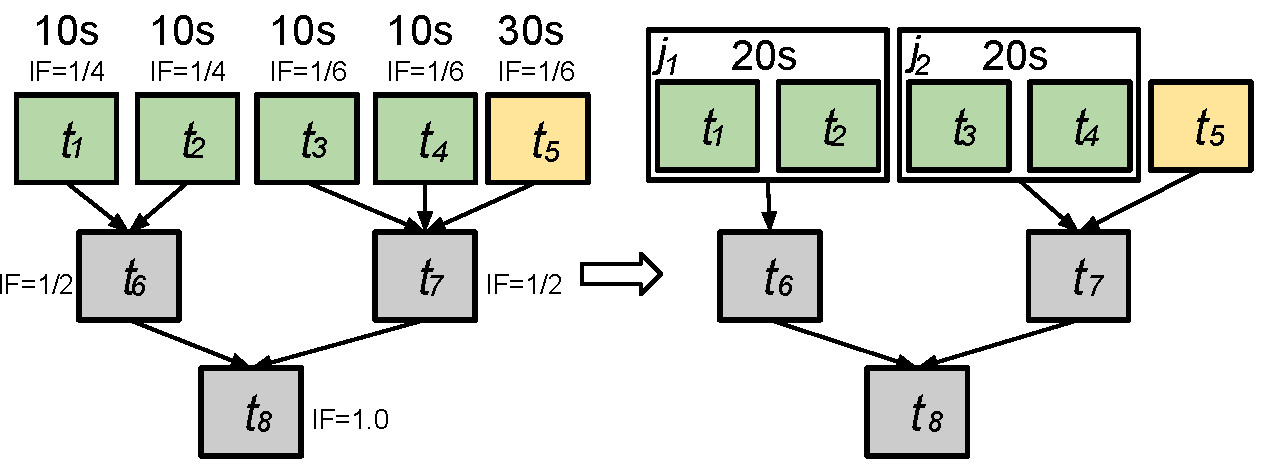
\includegraphics[width=\linewidth]{figures/imbalance/hifb.pdf}
	\captionof{figure}{An example of the HIFB (Horizontal Impact Factor Balancing) method. Impact factors allow the detection of similarities between tasks.}
	\label{fig:imbalance_hifb}
\end{figure}

However, HIFB is suitable for workflows with asymmetric structure. For symmetric workflows, such as the one shown in Figure~\ref{fig:imbalance_hrb}, the $IF$ value for all tasks of the first level will be the same ($IF=0.25$), thus the method may also cause dependency imbalance. In HDB, jobs are sorted based on the distance between them and the targeted task $t$, then on their runtimes. 
Algorithm~\ref{alg:imbalance_hdb} shows the pseudo codes of HDB. 
For instance, in Figure~\ref{fig:imbalance_hdb}, the distances between tasks $D(t_1,t_2)=D(t_3,t_4)=2$, while $D(t_1,t_3)=D(t_1,t_4)=D(t_2,t_3)=D(t_2,t_4)=4$. Thus, HDB merges a list of candidate tasks with the minimal distance ($t_1$ and $t_2$, and $t_3$ and $t_4$). Note that even if the workflow is asymmetric (Figure~\ref{fig:imbalance_hifb}), HDB would obtain the same result as with HIFB. 

\begin{figure}[!htb]
	\centering
	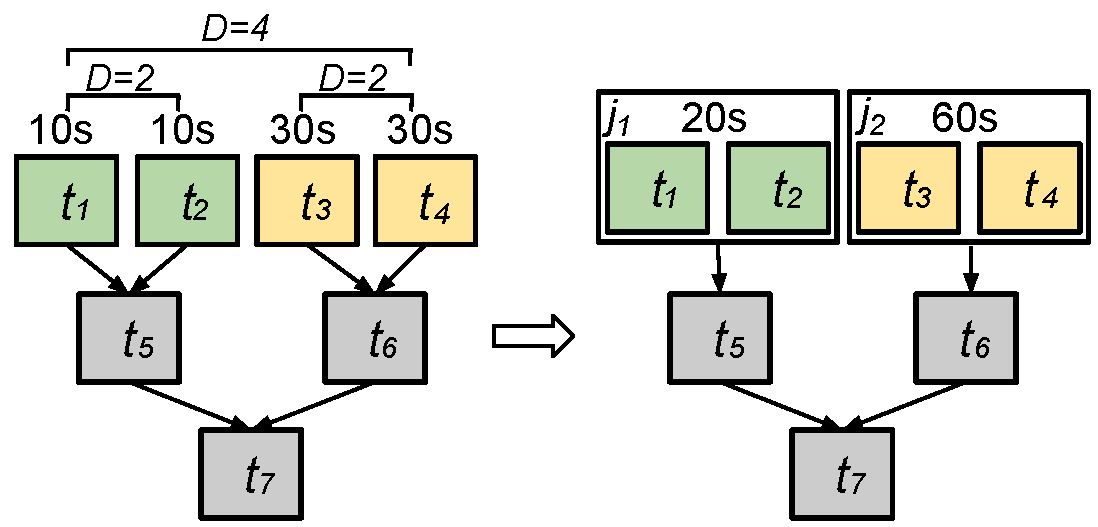
\includegraphics[width=0.85\linewidth]{figures/imbalance/hdb.pdf}
	\captionof{figure}{An example of the HDB (Horizontal Distance Balancing) method. Measuring the distances between tasks avoids data locality problems.}
	\label{fig:imbalance_hdb}
\end{figure}

There are cases where HDB would yield lower performance than HIFB. For instance, let $t_1$, $t_2$, $t_3$, $t_4$, and $t_5$ be the set of tasks to be merged in the workflow presented in Figure~\ref{fig:imbalance_hifb_hdb}. HDB does not identify the difference in the number of parent/child tasks between the tasks, since $d(t_u,t_v) = 2, \forall u,v \in [1,5], u \neq v$. On the other hand, HIFB does distinguish them since their impact factors are slightly different. Example of such scientific workflows include the LIGO Inspiral workflow~\cite{LIGO}, which is used in the evaluation of this work (Section~\ref{sec:results}).

\begin{figure}[!htb]
	\centering
	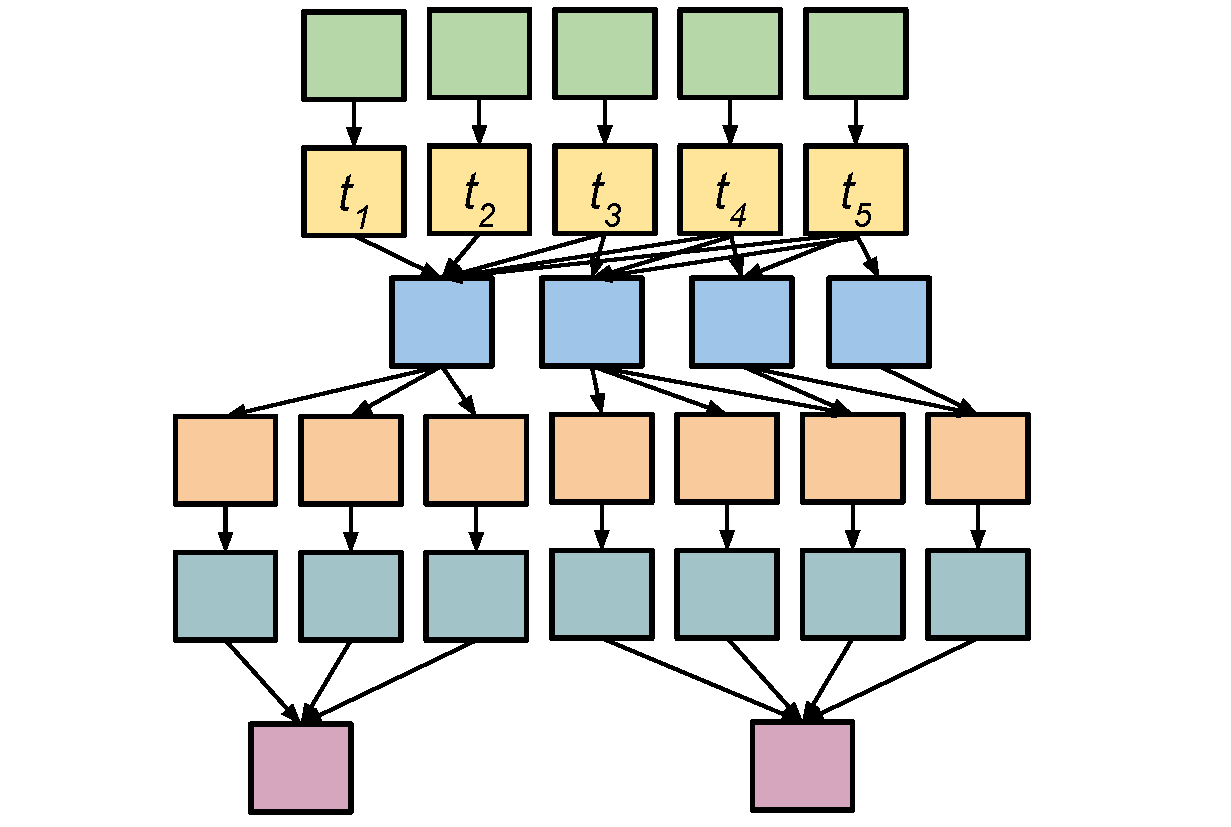
\includegraphics[width=0.85\linewidth]{figures/imbalance/hifb_vs_hdb.pdf}
	\captionof{figure}{A workflow example where HDB yields lower performance than HIFB. HDB does not capture the difference in the number of parents/child tasks, since the distances between tasks ($t_1$, $t_2$, $t_3$, $t_4$, and $t_5$) are the same.}
	\label{fig:imbalance_hifb_hdb}
\end{figure}

%In conclusion, these balancing methods have different preference on the selection of a candidate job to be merged with the targeting task. HIFB tends to group tasks that share similar position/importance to the workflow structure. HDB tends to group tasks that are closed to each other to reduce data transfers. 
Table~\ref{tab:2} summarizes the imbalance metrics and balancing methods presented in this work. 

\begin{figure}[htb]
	\centering
	\small
	\begin{tabular}{l|l}
		\hline
		\textbf{Imbalance Metrics} & $abbr.$   \\
		\hline
		Horizontal Runtime Variance & \emph{HRV}   \\ 
%		%Pipeline Runtime Variance &{\em PRV}  \\ 
		Horizontal Impact Factor Variance & \emph{HIFV} \\ 
		Horizontal Distance Variance & \emph{HDV}  \\ 
		\hline
		\textbf{Balancing Methods} & $abbr.$  \\
		\hline
%		Horizontal Clustering & HC \\
		Horizontal Runtime Balancing & HRB   \\ 
%		Vertical Clustering & VC \\ 
		Horizontal Impact Factor Balancing & HIFB\\ 
		Horizontal Distance Balancing & HDB \\ 
		\hline
	\end{tabular}
	\captionof{table}{Summary of imbalance metrics and balancing methods.}
	\label{tab:2}
\end{figure}



\subsection{Combining vertical clustering methods}

In this subsection, we discuss how we combine the balanced clustering methods presented above with vertical clustering (VC).
%For one example workflow shown in Figure~\ref{fig:imbalance_vc}, we may simply merge tasks at the fourth level and tasks at the fifth level vertically. 
In pipelined workflows (single-parent-single-child tasks), vertical clustering always yields improvement over a baseline, non-clustered execution because the merging reduces system overheads and data transfers within the pipeline. Horizontal clustering does not have the same guarantee since its performance depends on the comparison of system overheads and task durations. However, vertical clustering has limited performance improvement if the workflow does not have pipelines. Therefore, we are interested in the analysis of the performance impact of applying both vertical and horizontal clustering in the same workflow. We combine these methods in two ways: (\emph{i}) \emph{VC-prior}, and (\emph{ii}) \emph{VC-posterior}.


%\label{sec:vertical}
%\begin{figure}[htb]
%	\centering
%	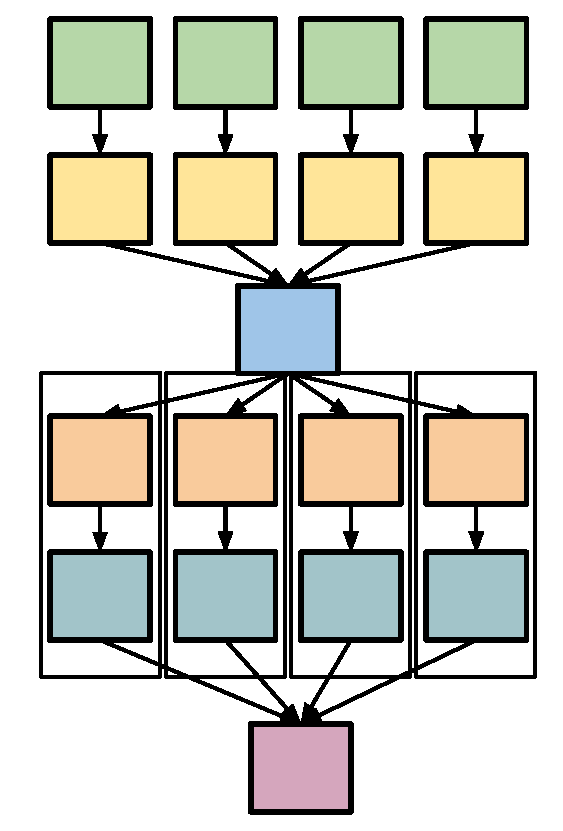
\includegraphics[width=0.35\linewidth]{figures/imbalance/vertical_clustering.pdf}
%	\captionof{figure}{An example of Vertical Clustering.}
%	\label{fig:imbalance_vc}
%\end{figure}

\paragraph{\textbf{VC-prior}}
In this method, vertical clustering is performed first, and then the balancing methods (HRB, HIFB, HDB, or HC) are applied. Figure~\ref{fig:imbalance_vc_prior} shows an example where pipelined-tasks are merged first, and then the merged pipelines are horizontally clustered based on the runtime variance.

\begin{figure}[!htb]
	\centering
	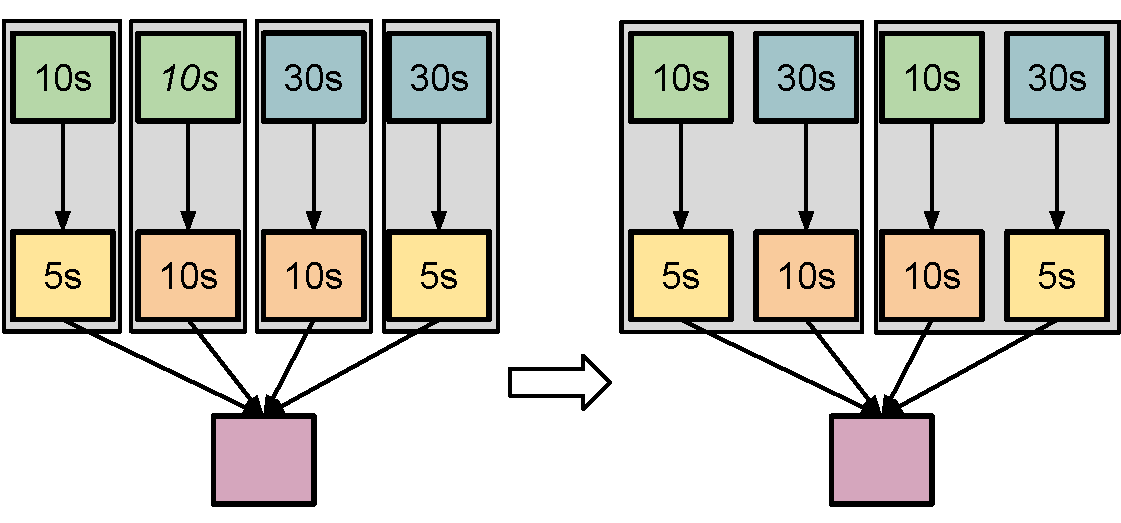
\includegraphics[width=0.85\linewidth]{figures/imbalance/vertical_clustering_prior.pdf}
	\captionof{figure}{\emph{VC-prior}: vertical clustering is performed first, and then the balancing methods.}
	\label{fig:imbalance_vc_prior}
\end{figure}

\paragraph{\textbf{VC-posterior}} 
%Here, vertical clustering is performed \emph{a posteriori}, i.e. balancing methods are first applied, and then VC. Figure~\ref{fig:imbalance_vc_posterior} shows an example where tasks are horizontally clustered first based on the runtime variance, and then merged vertically. In this example, vertical clustering targeted the data locality problem by merging tasks that would not generate interdependency once clustered. However, this approach causes a runtime imbalance problem.

\begin{figure}[!htb]
	\centering
	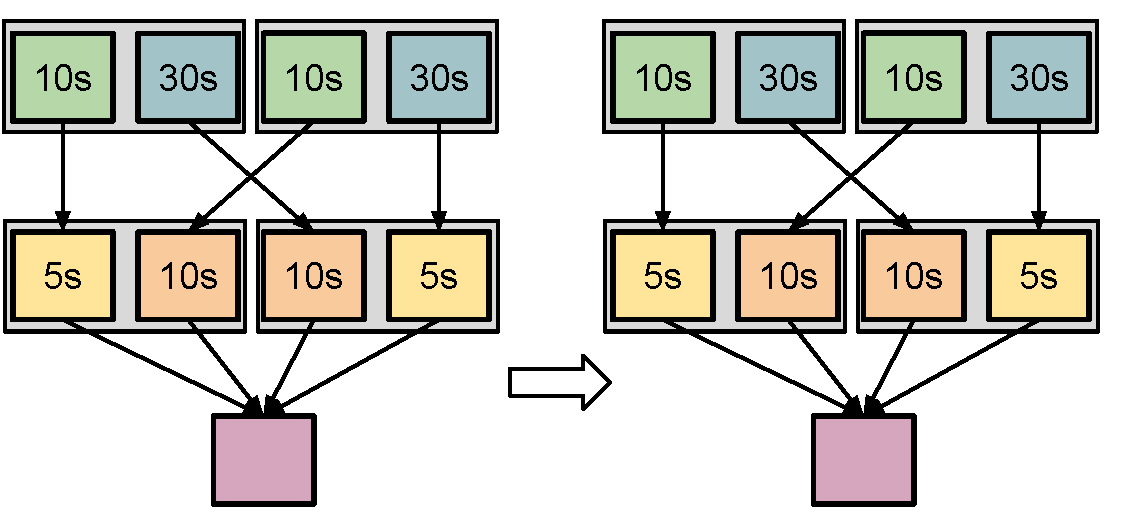
\includegraphics[width=0.85\linewidth]{figures/imbalance/vertical_clustering_posterior3.pdf}
	\captionof{figure}{\emph{VC-posterior}: horizontal clustering (balancing methods) is performed first, and then vertical clustering.}
	\label{fig:imbalance_vc_posterior}
\end{figure}

Here, balancing methods are first applied, and then vertical clustering. Figure~\ref{fig:imbalance_vc_posterior} shows an example where tasks are horizontally clustered first based on the runtime variance, and then merged vertically. However, since the original pipeline structures have been broken by horizontal clustering, VC does not perform any changes to the workflow. 


%means we perform horizontal clustering methods first and then vertical clustering. For the same workflow, assuming we merge tasks horizontally as shown in , we can see that we cannot perform vertical clustering to clustered jobs at the fourth level and the fifth level since the original pipeline structures have been destroyed by horizontal clustering. This phenomenon suggests us VC-posterior may work better compared to VC-prior, generally speaking. However, some opposite cases do exist. We will verify our hypothesis in Section~\ref{sec:results}. We will also compared the two combining approaches with \textbf{VC-only}, which means we perform vertical clustering only and \textbf{No-VC}, which means we just perform horizontal clustering methods without vertical clustering. 








\section{Sensitivity Metrics}
\label{sec:sensitivity}
\subsection{Introduction}


Many computational scientists develop and use large-scale, loosely-coupled applications that are often structured as scientific workflows, which consist of many computational tasks with data dependencies between them. When executing these applications on a multi-machine distributed environment, such as the Grid or the Cloud, significant system overheads may exist~\cite{Chen2011, Prodan2008b, Dong2010, Yang03, WorkflowSim} and the problem of choosing robust schedules becomes more and more important. Traditionally, a carefully crafted schedule is based on deterministic or statistic estimates for the execution time of computational activities that compose a workflow. However, in such an environment, this approach may prove to be grossly inefficient~\cite{WorkflowSim}, as a result of various unpredictable overheads that may occur at runtime. 
%Particularly, it is challenging to provide a good estimate of overheads since it involves a lot of uncertainties. 
Thus, to mitigate the impact of uncertain overheads, it is necessary to choose a schedule that guarantees overhead robustness, that is, a schedule that is affected as little as possible by various overhead changes.  

There are several ways to achieve overhead robustness. A first approach is to integrate the overhead estimation into the job scheduling problem. A static or statistic estimation of communication cost or data transfer delay~\cite{Dong2010, Yang03} has been considered in the scheduling problem. Once we have the deterministic or statistic information of overheads, we can treat the system overhead as computational activities and the goal is to minimize the overall runtime including overhead duration. However, this approach only applies to the estimation of data transfer delay since the highly unpredictable variability and variety of other overheads make it a challenging work and not efficient in practice. Our prior work~\cite{Chen} has shown the variation of overheads may be comparable to the job runtime and thus makes it unrealistic in a real environment.  

A significant amount of work~\cite{Ahmad1998, Chetto1990, Dong2010, Yang03} in the literature has focused on proposing algorithms that are aware of the dynamic changes of runtime environments. Task rescheduling~\cite{Sakellariou2004, Zhang2009, Chen2010} is a typical approach that dynamically allocates tasks to an idle processor in order to take into account information that has been made available during the execution. Specifically, resource load~\cite{Dong2010} can be used to estimate the variance. However, rescheduling a task is costly as it implies some extra communication and synchronization costs. Relevant studies~\cite{Sakellariou2004} indicate that it is important to have a static schedule with good properties before the start of the execution. Therefore, even if a dynamic strategy is used, a good initial placement would reduce the possibility of making a bad decision. 

Another approach is to overestimate the execution time of individual jobs. Delay scheduling~\cite{Zaharia10} waits for a small amount of time, letting other MapReduce jobs launch tasks instead and this method can achieve a better tradeoff of locality and fairness. However, this method only applies to workload scheduling and particularly MapReduce jobs since the duration of them is short and thus it is not difficult to estimate the scheduling delay. Also, this results in a waste of resources as it induces a lot of idle time during the execution, if the overhead is shorter than the estimation. Second, overheads do not simply work as an attachment to the job runtime and it involves a lot more complicated patterns such as periodicity~\cite{Chen}. 

In this paper, we first present our work on evaluating the overhead robustness of scheduling heuristics and we indicate a list of heuristics that are overhead robust even without an estimate of the overhead duration. Second, since the estimate of overhead duration is difficult, we develop new heuristics that leverage the pattern information of workflow overheads, which represents a new approach to design overhead robust algorithms. To the best of our knowledge, so far, no study has systematically tried to evaluate the scheduling heuristics with respect to the overhead robustness.  



%Braun paper
%Opportunistic Load Balancing, Minimum Execution Time, Minimum Completion Time, Min-min, Max-min, Duplex, Genetic Algorithm, Simulated Annealing, Genetic Simulated Annealing, Tabu, and A*

%The 11 static mapping heuristics were evaluated using simulated execution times for an HC environment. Because these are static heuristics, it is assumed that an accurate estimate of the expected execution time for each task on each machine is known prior to execution and contained within a  ETC (expected time to compute) matrix. The assumption that these estimated expected execution times are known is commonly made when studying mapping heuristics for HC systems (e.g., [19, 26, 40]). (Approaches for doing this estimation based on task profiling and analytical benchmarking are discussed in [27, 30, 37].)


\subsection{Overhead Patterns}

In this section, we introduce the common overhead patterns in workflow execution. 
In scientific workflow systems, time related functionalities such as workflow scheduling normally requires effective forecasting of activity patterns. In this work, we mainly focus on the overhead pattern that refers to a representative time series of overhead activities that occurs repeatedly and regularly in workflow execution. An overhead pattern is composed of ordered overhead activities obtained from scientific workflow system logs or other forms of historical data. 
Pattern discovery~\cite{Liu2008} usually starts from a periodical sampling plan to build representative duration series (Job Release, etc. ) and then conducts time-series segmentation to discover the pattern sets and predicts the activity duration intervals with pattern matching results. 


The motivation for pattern based analysis comes from the observation that for those duration-series segments where the number of concurrent activity instances is similar, these activity durations reveal comparable statistical features. Due to the dynamic nature of underlying resources, pattern based forecasting of overheads can improve the effectiveness of scheduling heuristics. 

\begin{figure}[htb]
\centering
 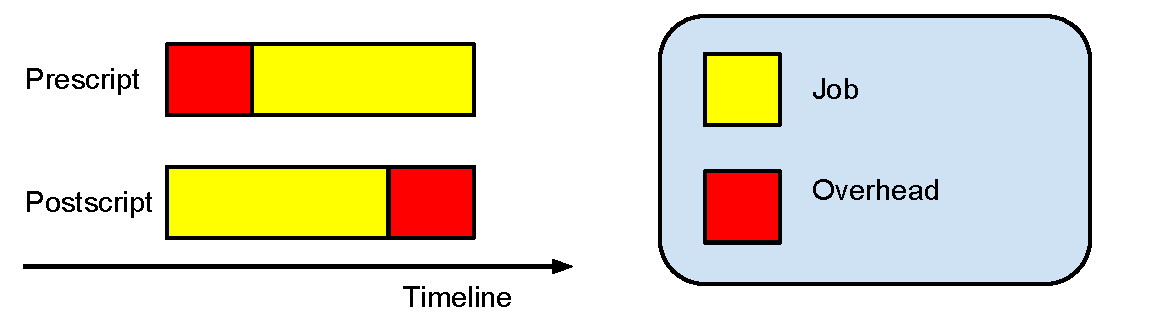
\includegraphics[width=1\linewidth]{figure/adherence.pdf}
  \captionof{figure}{Adherence Pattern}
  \label{fig:adhere}
  \vspace{-10pt}
\end{figure}

Most of the work~\cite{Dong2010, Yang03} view the overhead duration as an attachment to runtime in workflow timeline. For example, the Pre/Post-script Delay is usually constant, which we call it Adherence Pattern as shown in Fig.~\ref{fig:adhere}. Scheduling algorithms can just add the delay to the job runtime without significant change to the algorithms. For this pattern, we have shown in our prior work~\cite{Chen} that it does not have much influence on the overhead robustness. 
However, we observe that the Workflow Engine Delay and the Queue Delay increases periodically and steadily. For example, Fig.~\ref{fig:trace} shows the Gantt chart of part of a real trace\footnote{Details: http://www.isi.edu/\string~wchen/fgrid/run}. 
The Workflow Engine Delay (red) of the first 16 jobs is 5 seconds and then it increases to 10 seconds. 
%It is difficult to explain queue delay
We call this common overhead pattern the Incremental and Periodical Pattern (IPP). We observe the Queue Delay also increases periodically but the period is interrupted by the resource availability and thus it has a more complicated IPP. In the rest of this paper, we focus on the IPP of the Workflow Engine Delay and we will cover the Queue Delay in our future work. 
The reason why IPP prevalently exists is that many workflow management components are queue based systems. They repeatedly check their queues to find whether there are idle jobs, if yes they will process and submit these jobs, otherwise it will wait for a interval and continue. In Fig.~\ref{fig:ipp} we abstract the IPP from the trace, which shows a repeatedly increase by a interval. We define throughput of a workflow management component as the maximum number of allowed jobs in queue. For example, the interval and the throughput of the Workflow Engine in Fig.~\ref{fig:trace} are around 5 seconds and 16 respectively. 


\begin{figure}[htb]
\centering
 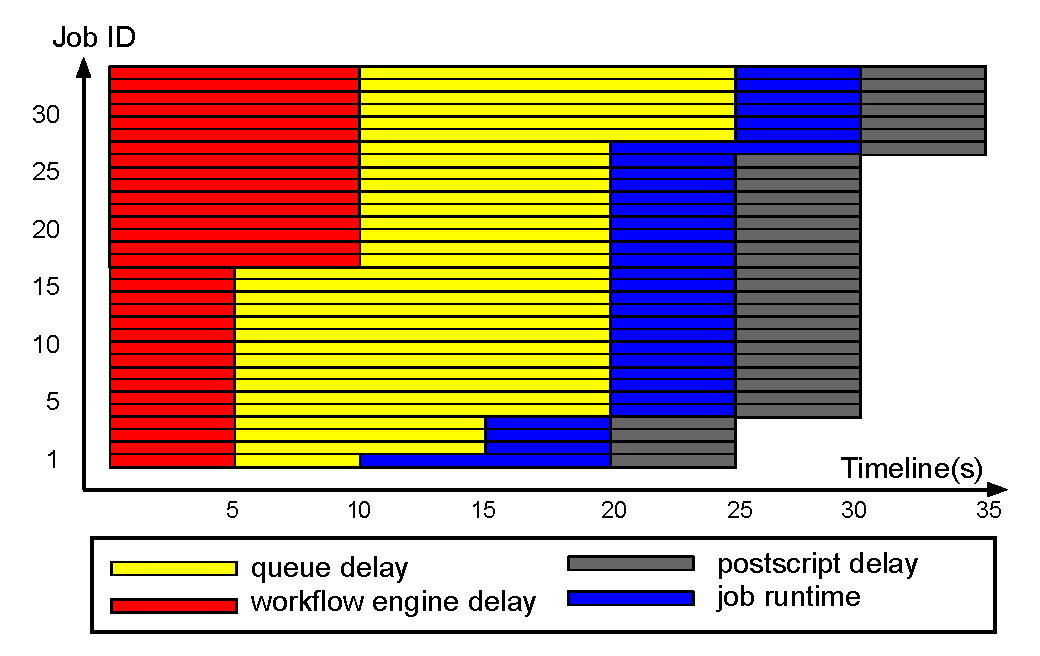
\includegraphics[width=1\linewidth]{figure/trace.pdf}
  \captionof{figure}{Workflow Execution Gantt Chart of a Real Trace}
  \label{fig:trace}
  \vspace{-10pt}
\end{figure}



%Some representative time series, including marketing time series, temperature time series and quality control time series, are effectively applied in various scientific and business domains [6][7]. Similarly, 

%Current forecasting strategies for computation tasks mainly reside on the prediction of CPU load [1][15], however, this is quite different from the prediction of scientific workflow activity durations.Activity durations cover the time intervals from the initial submission to the final completion of each workflow activity [3]. Hence, besides the exact execution time on scheduled resources, they also consist of extra time, i.e. scientific workflow overheads. According to [11], there exist four main categories of scientific workflow overheads, i.e. middleware overhead, data transfer overhead, loss of parallelism overhead and activity related overhead. Evidently, scientific workflow activity durations involve much more affecting factors than that of conventional computation tasks which are dominated by high performance computing resources.scientific workflow activity durations denote discrete long-term intervals since activity instances only occur occasionally and take several minutes or more than a couple of hours to complete.

%The motivation for pattern based time-series forecasting comes from the observation that for those duration-series segments where the number of concurrent activity instances is similar, these activity durations reveal comparable statistical features. 

These overhead patterns reappear frequently during a duration series and they represent unique behavior of the workflow management components. After we define and discover these typical patterns, the intervals and throughputs of these patterns can be estimated and statistically captured from historical traces. 



%Furthermore, if these overhead patterns reappear frequently during a duration series, they can be deemed as potential patterns which represent unique behavior of the duration-series under certain circumstances. Therefore, if we are able to define and discover these typical patterns, the intervals of future durations can be estimated with the statistical features of the closest patterns by matching the latest duration sequences. 





\begin{figure}[htb]
\centering
 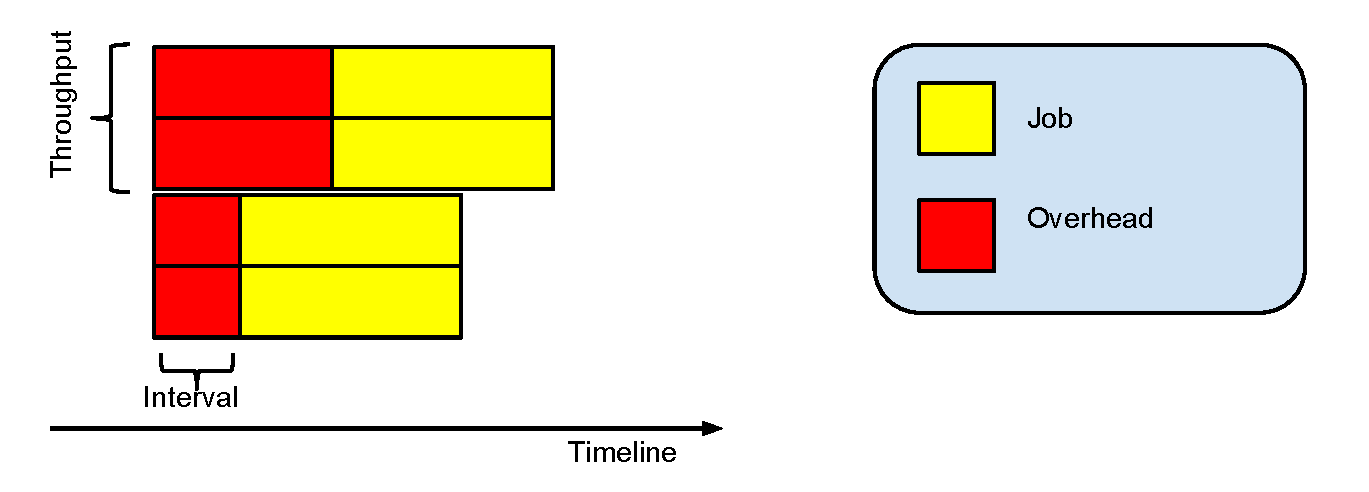
\includegraphics[width=1\linewidth]{figure/incremental.pdf}
  \captionof{figure}{Incremental and Periodical Pattern}
  \label{fig:ipp}
  \vspace{-10pt}
\end{figure}

%It is not workflow engine delay it is workflow engine interval
\section{Overhead Robust Heuristics}
\label{sec:heuristics}
In this section, we introduce the overhead robustness of four pairs of scheduling heuristics. Heuristics are widely used in workflow scheduling since the scheduling problem is a NP-hard problem and the time complicity of a global optimization of the overall runtime is not affordable. Usually, heuristics utilize unique features of workflows or resources to guide the mapping of jobs to resources. For example, both of the MINMIN~\cite{Blythe2005} algorithm and the MAXMIN~\cite{Braun2001} algorithm utilize the runtime of a job as the feature. However, they conduct the mapping in an opposite way, that is, MINMIN chooses the job with the shortest runtime while MAXMIN chooses the job with the longest runtime. Intuitively speaking, there must be either of them (we call it overhead robust) that performs better than the other one (we call it overhead unrobust) since they operates oppositely. Inspired by these coupling heuristics, we use a relative overhead robustness approach to evaluate these scheduling heuristics. For a pair of heuristics that use the same feature, we define the relative overhead robustness as the performance gain of the overhead robust heuristic against the other one. The more performance gain we have, the more significant this feature has on the overhead robustness. Also, it is not fair to compare scheduling heuristics that use different features because they may have vastly different performance even without overheads. Furthermore, in practice, we can use scheduling heuristics with different features at the same time but not those with the same features. 
Below we introduce the four pairs of scheduling heuristics including one that we propose. 

%OLB: Opportunistic Load Balancing (OLB) assigns each task, in arbitrary order, to the next machine that is expected to be available, regardless of the task's expected execution time on that machine [3, 17, 18]. The intuition behind OLB is to keep all machines as busy as possible. One advantage of OLB is its simplicity, but because OLB does not consider expected task execution times, the mappings it finds can result in very poor makespans.
%MET: In contrast to OLB, Minimum Execution Time ( MET ) assigns each task, in arbitrary order, to the machine with the best expected execution time for that task, regardless of that machine's availability [3, 17]. The motivation behind MET is to give each task to its best machine. This can cause a severe load imbalance across machines. In general, this heuristic is obviously not applicable to HC environments characterized by consistent ETC matrices.
%MCT: Minimum Completion Time (MCT) assigns each task, in arbitrary order, to the machine with the minimum expected completion time for that task [3]. This causes some tasks to be assigned to machines that do not have the minimum execution time for them. The intuition behind MCT is to combine the benefits of OLB and MET, while avoiding the circumstances in which OLB and MET perform poorly.

\emph{MINMIN} and \emph{MAXMIN}: The MINMIN heuristic begins with a set of all unmapped jobs. Then, the set of minimum completion times for each job, M namely, is found. Next, the job with the overall minimum completion time from M is selected and assigned to the corresponding resource (hence the name MINMIN). Last, the newly mapped job is removed from the unmapped jobs, and the process repeats until all jobs are mapped. 
%Minin maps the tasks in the order that changes the machine availability status by the least amount that any assignment could. Let ti be the first task mapped by Minin onto an empty system. The machine that finishes ti the earliest, say mj , is also the machine that executes ti the fastest. For every task that MINMIN maps after ti, the Minin heuristic changes the availability status of mj by the least possible amount for every assignment. Therefore, the percentage of tasks assigned to their first choice (on the basis of execution time) is likely to be higher for Minmin than for Maxin (defined next). The expectation is that a smaller makespan can be obtained if more tasks are assigned to the machines that complete them the earliest and also execute them the fastest.
The MAXMIN heuristic is very similar to MINMIN. The MAXMIN heuristic also begins with the set of all unmapped jobs. Then, the set of minimum completion times, M, is found. Next, the job with the overall maximum completion time from M is selected and assigned to the corresponding resource (hence the name MAXMIN). Last, the newly mapped job is removed from the unmapped jobs, and the process repeats until all jobs are mapped. 
Intuitively speaking, we believe MAXMIN has better overhead robustness than MINMIN. As shown in Fig.~\ref{fig:longest}, assuming we have two jobs and the interval of the overhead is 1. MAXMIN releases a job with longer runtime first, which can overlap with the increment of the overheads when MAXMIN releases the other job. However, the performance gain depends on the values of overhead interval, job runtime, overhead duration and the resource availability. 

\begin{figure}[htb]
\centering
 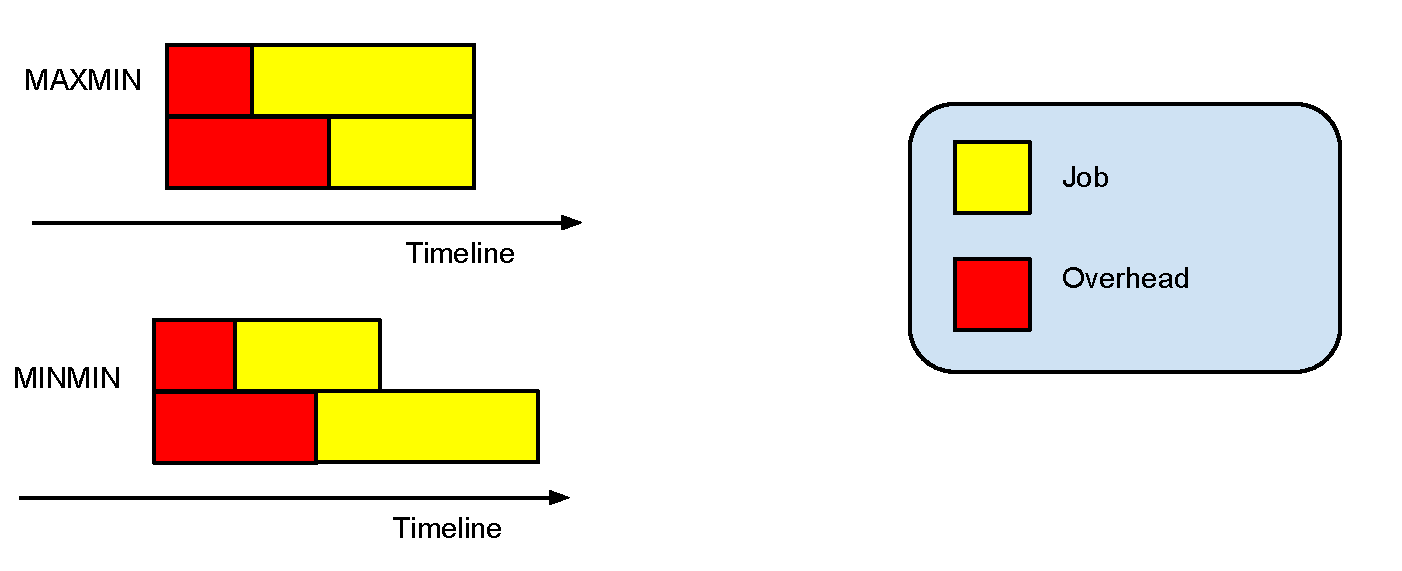
\includegraphics[width=1.0\linewidth]{figure/longest.pdf}
  \captionof{figure}{MAXMIN vs. MINMIN}
  \label{fig:longest}
  \vspace{-10pt}
\end{figure}
\emph{Breadth First} and \emph{Depth First}: Namely, the Breadth First (BFS) algorithm iterates the jobs at the same workflow level (or depth within a workflow directed acyclic graph) first while the Depth First (DFS) algorithm iterates the jobs at the deepest workflow level first. Intuitively speaking, we believe BFS performs better than DFS in terms of overhead robustness since BFS releases more jobs at the same workflow level for most scientific workflows as shown in Fig.~\ref{fig:shape}. Therefore, with enough jobs in queue, BFS can fully utilize the resources without wasting this overhead interval.  

\emph{Fertile First} and \emph{Unfertile First}: The Fertile First (FFS) algorithm sorts all the unmapped jobs based on the number of children jobs that they have and assigns the jobs with most children jobs first. The Unfertile First (UFFS) algorithm works in the opposite way and assigns the jobs with lest children jobs first. Similar to the case of BFS and DFS, we believe FFS should perform better than UFFS since FFS releases more jobs at the next level compared to UFFS and thus FFS can fully utilize the available resources. 

\begin{figure}[htb]
\centering
 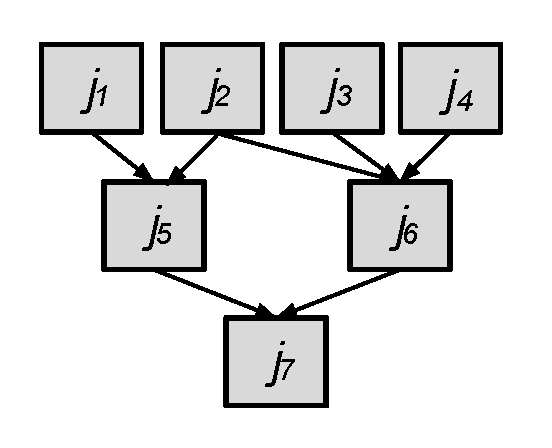
\includegraphics[width=0.6\linewidth]{figure/impact_factor.pdf}
  \captionof{figure}{Impact Factor}
  \label{fig:impact}
  \vspace{-10pt}
\end{figure}

\emph{Important First} and \emph{Unimportant First}: Here we propose a pair of Impact Factor based scheduling heuristics. The Important First (IFS) algorithm sorts all the unmapped jobs based on their \emph{Impact Factor} (IF) and assigns the jobs with the largest IF first while the Unimportant First (UIFS) algorithm assigns the jobs with the smallest IF first. 
The \textbf{Impact Factor} ($IF$) of a job $j_u$ is defined as follows:

\begin{equation}
	IF(j_u)=\sum_{j_v\in Child(j_u)}^{}\frac{IF(j_v)}{L(j_v)}
\end{equation}
where $Child(j_u)$ denotes the set of child jobs of $j_u$, and $L(j_v)$ the number of parent jobs of $j_v$. For simplicity, we assume the $IF$ of a workflow exit job (e.g. $j_7$ in Fig.~\ref{fig:impact}) as 1.0. For instance, consider the workflow in Fig.~\ref{fig:impact}. $IF$ for $j_1$, $j_2$, $j_3$, and $j_4$ are computed as follows:

\begin{eqnarray}
	\displaystyle  
	&IF(j_7 )=1.0, IF(j_6 )=IF(j_5 )=IF(j_7 )/2=0.5\nonumber  \\
	&IF(j_1 )=IF(j_5)/2=0.25\nonumber \\
	&IF(j_2 )=IF(j_5 )/2+IF(j_6)/3=0.42\nonumber \\
	&IF(j_3 )=IF(j_4 )=IF(j_6 )/3=0.17\nonumber 
\end{eqnarray}
Thus, IFS algorithm should schedule $j_2$ first while UIFS algorithm should schedule $j_3$ or $j_4$ first. The intuition of Impact Factor is that we aim to measure the relative importance of a job to the entire graph. Intuitively speaking, tasks with larger impact factors should have more impacts on the remaining jobs compared to tasks with smaller impact factors. For example, a bottleneck usually has a larger IF since it controls the release of more jobs. 
Similar to the case of FFS and UFFS, we believe IFS has a better overhead robustness than UIFS since IFS releases more jobs at the next few levels compared to UFFS. 


%The idea of these overhead aware heuristics is we would like to improve the overhead robustness even when we are not able to precisely predict the duration of overheads. Instead, workflow overheads have common patterns, which can determine the relative performance of different heuristics. 
Table~\ref{tab:heuristics} summaries the heuristics and their potential overhead robustness. 
\begin{table}[H]
\caption{Scheduling Heuristics}
\begin{center}
  \begin{tabular}{ l|l|l}
    \hline
Heuristics & Overhead Robust & Overhead Unrobust \\ \hline
    Experiment 1 & MAXMIN & MINMIN \\ \hline
   Experiment 2 & BFS & DFS \\ \hline
 Experiment 3 & FFS & UFFS \\ \hline
Experiment 4 & IFS & UIFS\\
    \hline
  \end{tabular}
\label{tab:heuristics}
\end{center}
\end{table}

% Section
\section{Experiment and Evaluation}


The experiments presented hereafter evaluate the performance of the four pairs of heuristics mentioned ahead, which are widely used by workflow management systems. 

\subsection{Experiment Conditions}


\begin{figure}[htb]
	\centering
	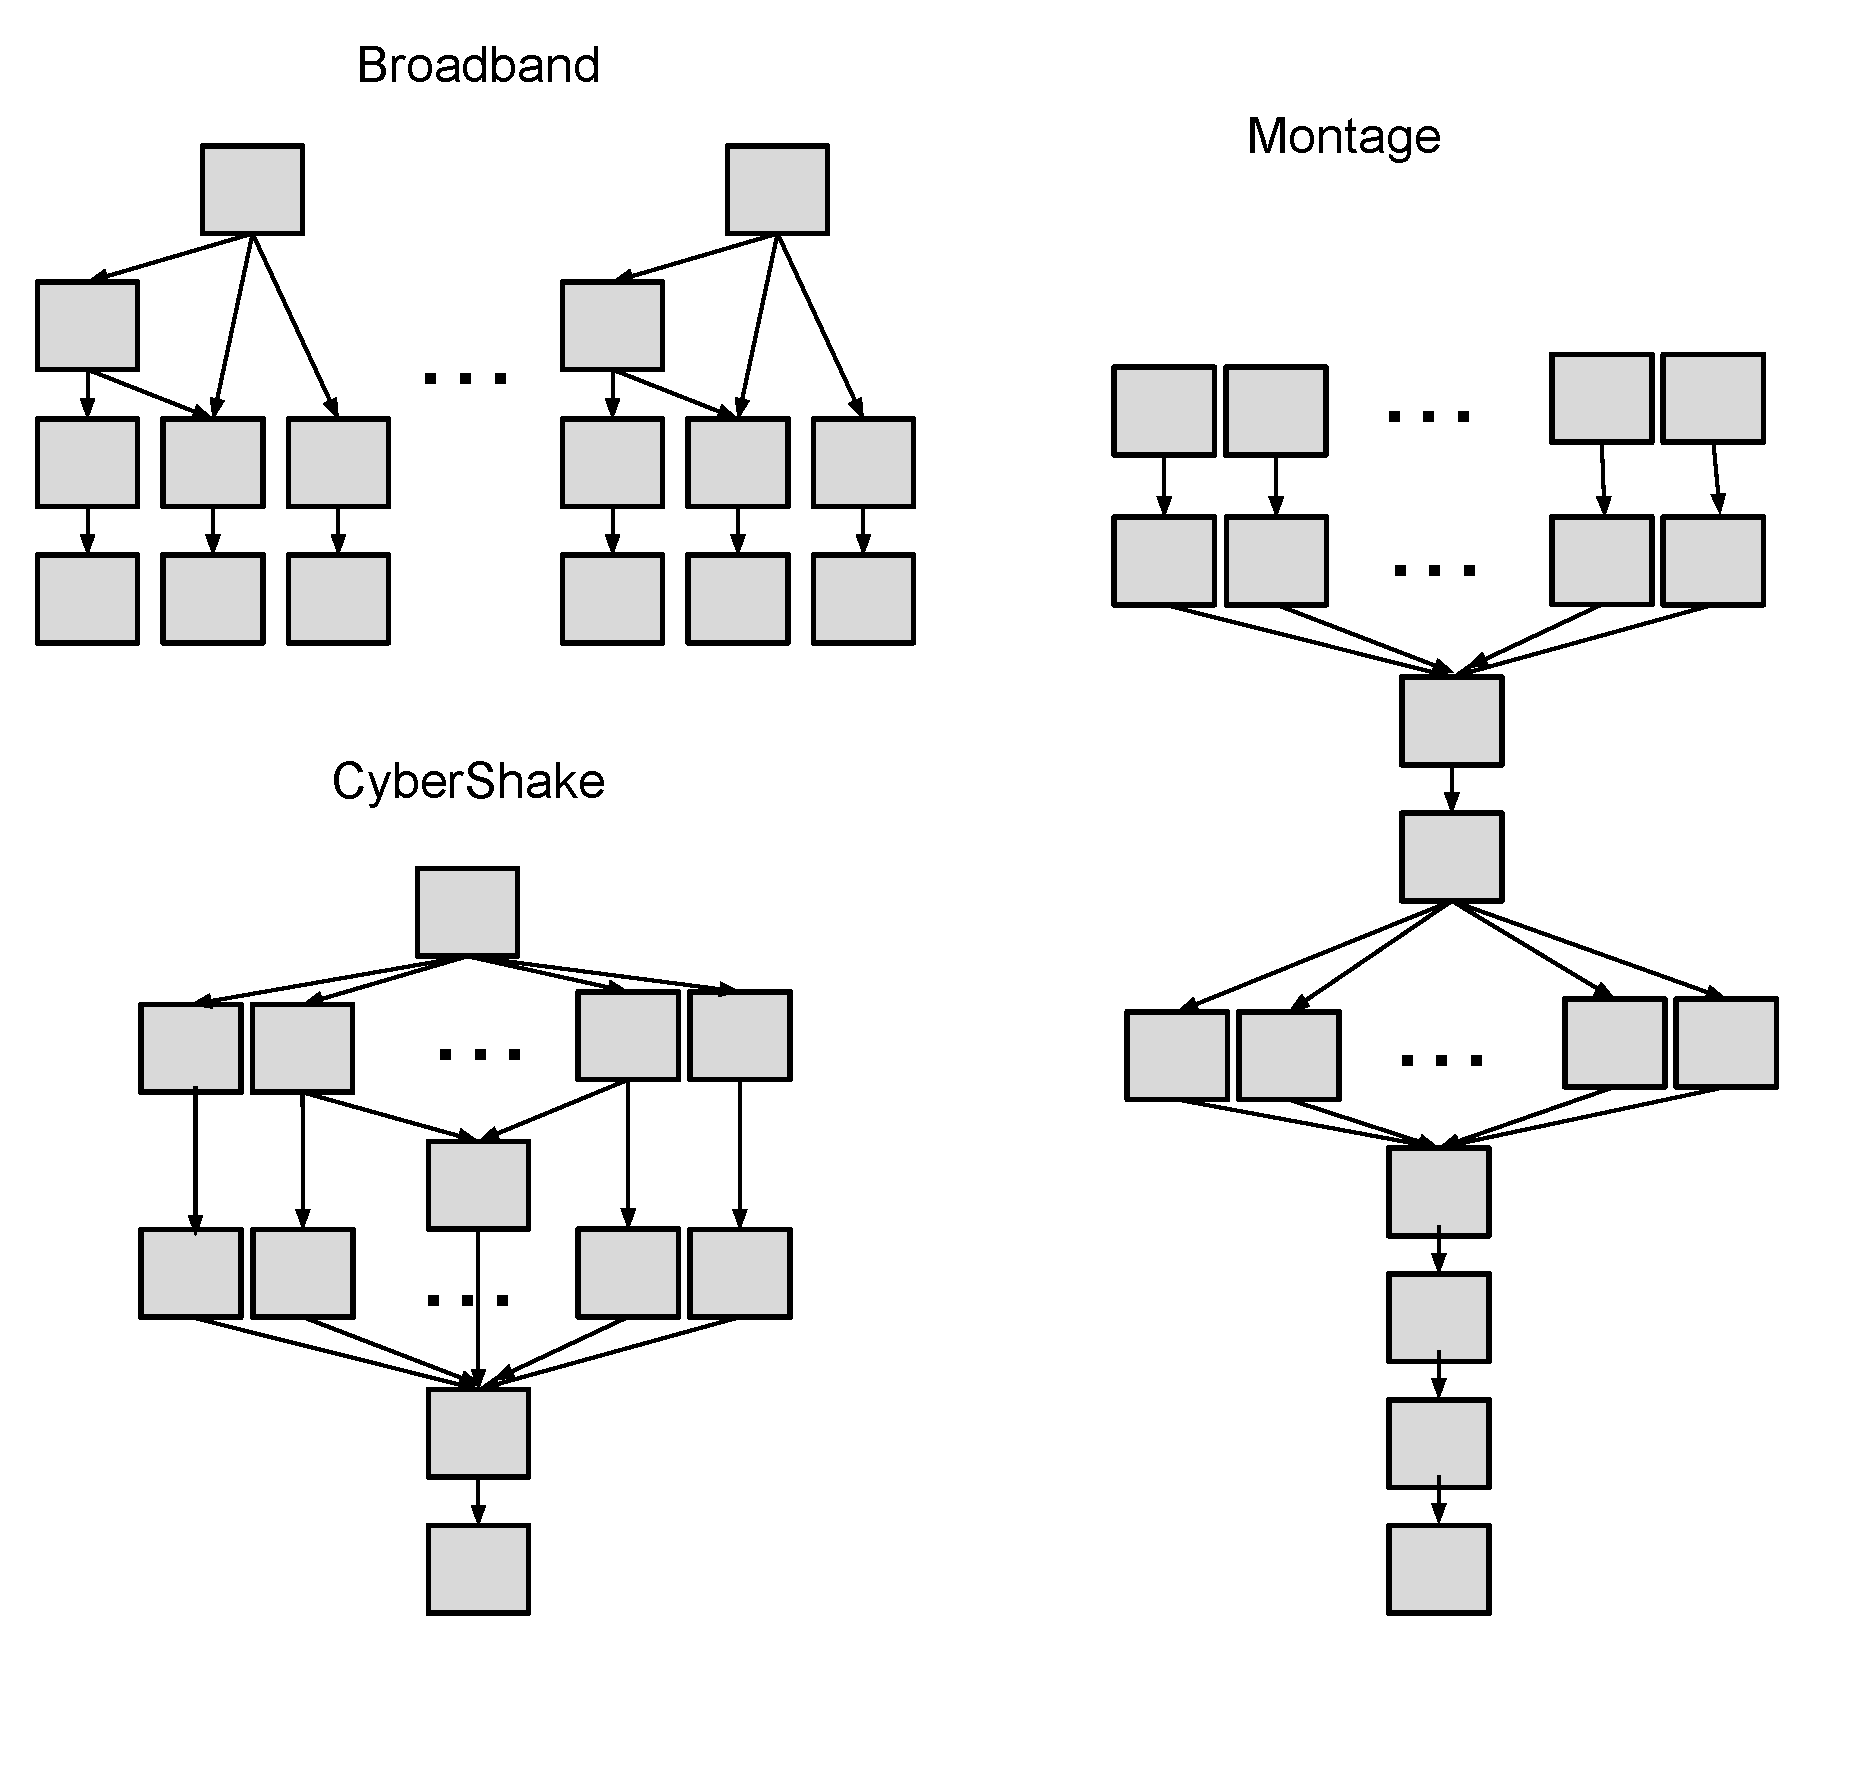
\includegraphics[width=1.0\linewidth]{figure/shape.pdf} 
	\caption{A simplified visualization of the Broadband workflow, the Montage workflow and the CyberShake workflow.}
	\label{fig:shape}
	\vspace{-10pt}
\end{figure}

We extended the WorkflowSim~\cite{WorkflowSim} simulator with the overhead model to simulate a distributed environment where we could evaluate the overhead robustness of scheduling algorithms when varying the average overheads and throughput. As an initial attempt, we focus on the workflow engine delay ($d$) in this paper. The simulated computing platform is composed by 20 single core virtual machines (worker nodes), which is the quota per user of some typical distributed environments such as Amazon EC2~\cite{AmazonAWS} and FutureGrid~\cite{FutureGrid}. Each machine has 512MB of memory and the capacity to process 1,000 million instructions per second. 
%Task scheduling is data-aware, i.e. tasks are scheduled to resources which have the most input data available.
%WorkflowSim is a feature-rich toolkit to simulate workflow planning and execution. It provides runtime randomization and multiple task clustering methods that we need. 



Three workflows are used in the experiments: 
Broadband~\cite{Broadband} is an application that enables researchers to combine long-period deterministic seismograms with high-frequency stochastic seismograms. 
Montage~\cite{Sakellariou2010} is an astronomy application used to construct large image mosaics of the sky. CyberShake~\cite{Callaghan2008} is a seismology application that calculates Probabilistic Seismic Hazard curves for geographic sites in the Southern California region. All workflows are generated and varied using the WorkflowGenerator\footnote[1]{https://confluence.pegasus.isi.edu/display/pegasus/WorkflowGenerator}. Each workflow instance is composed by around 100 tasks and its workflow structure is presented in Fig.~\ref{fig:shape}. Runtime (average and task runtime distribution) and overhead (workflow engine delay and queue delay) information were collected from real traces production environments~\cite{Chen2011, Juve2013}, then used as input parameters for the simulations.

%We first collected runtime information  (i.e., average and distribution of task runtime) and overhead information (including workflow engine delay, queue delay and network bandwidth) from the real traces that were run on real environments before. 
%Part of runtime distribution and overhead information were shown in \cite{Juve2013} and \cite{Chen} respectively. 
%Then we input these parameters into WorkflowSim and run these workflows repeatedly until the variance is less than 5\% of the average workflow runtime. 



Four sets of experiments are conducted. Experiment 1 evaluates the relative robustness of MAXMIN and MINMIN by comparing the performance gain of the overhead robust heuristic (MAXMIN in this experiment) over the overhead unrobust heuristic (MINMIN), while varying the average interval of workflow engine ($d$) and throughput of workflow engine ($t$). Table~\ref{tab:heuristics} shows the heuristics compared in these experiments. Simulation results present a confidence level of 95\%. Thus, for values of \emph{Performance Gain} $> 0$, the overhead robust heuristics perform better than the respective overhead unrobust heuristics. Otherwise, the overhead robust heuristics perform poorer.
%We randomly select 20\% from LIGO workflow tasks and increase their task runtime by a factor of \emph{Ratio} to simulate the system variation in a production environment.




In these experiment sets, we vary the average throughput of workflow engine from 1 to 20 and we show the results of $t=1, 5, 15, 20$. The original throughput of workflow engine in these traces is 5 and a throughput that is larger than 20 does not influence the performance much since we have only 20 worker nodes in our experiments. We also vary the average interval of workflow engine from 0 to 100 seconds, which represents a typical range of workflow engine delay as shown in~\cite{Chen2011} and this range is able to show the difference of overhead robustness in these heuristics. 

\subsection{Results and Discussion}

\begin{figure}[!htb]
\centering
 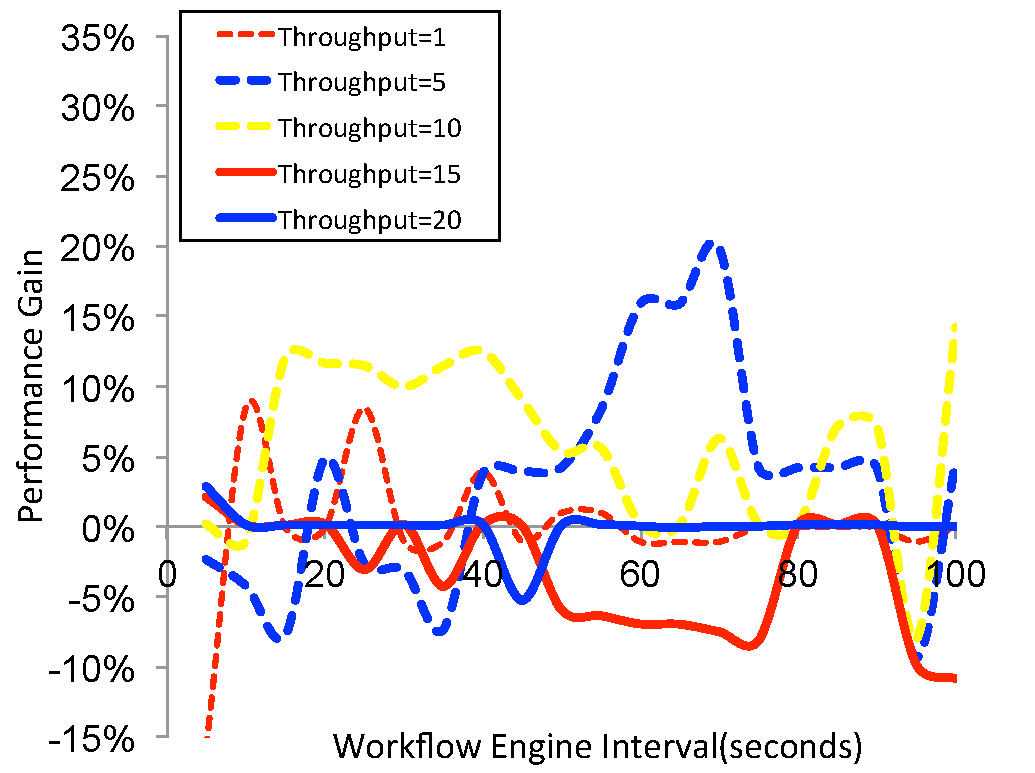
\includegraphics[width=0.9\linewidth]{figure/MAX-MIN-Broadband.pdf}
  \captionof{figure}{Broadband }
  \label{fig:MAX-MIN-Broadband}
  \vspace{-10pt}
\end{figure}

\begin{figure}[!htb]
\centering
 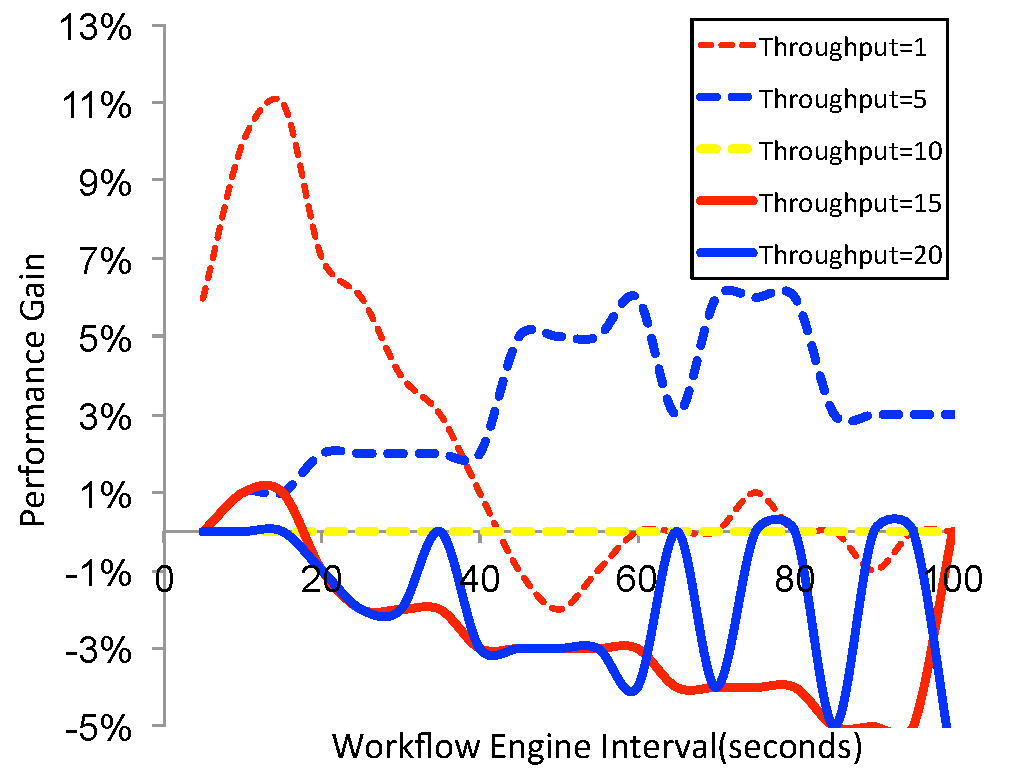
\includegraphics[width=0.9\linewidth]{figure/MAX-MIN-CyberShake.pdf}
  \captionof{figure}{CyberShake}
  \label{fig:MAX-MIN-CyberShake}
  \vspace{-10pt}
\end{figure}

\begin{figure}[!htb]
\centering
 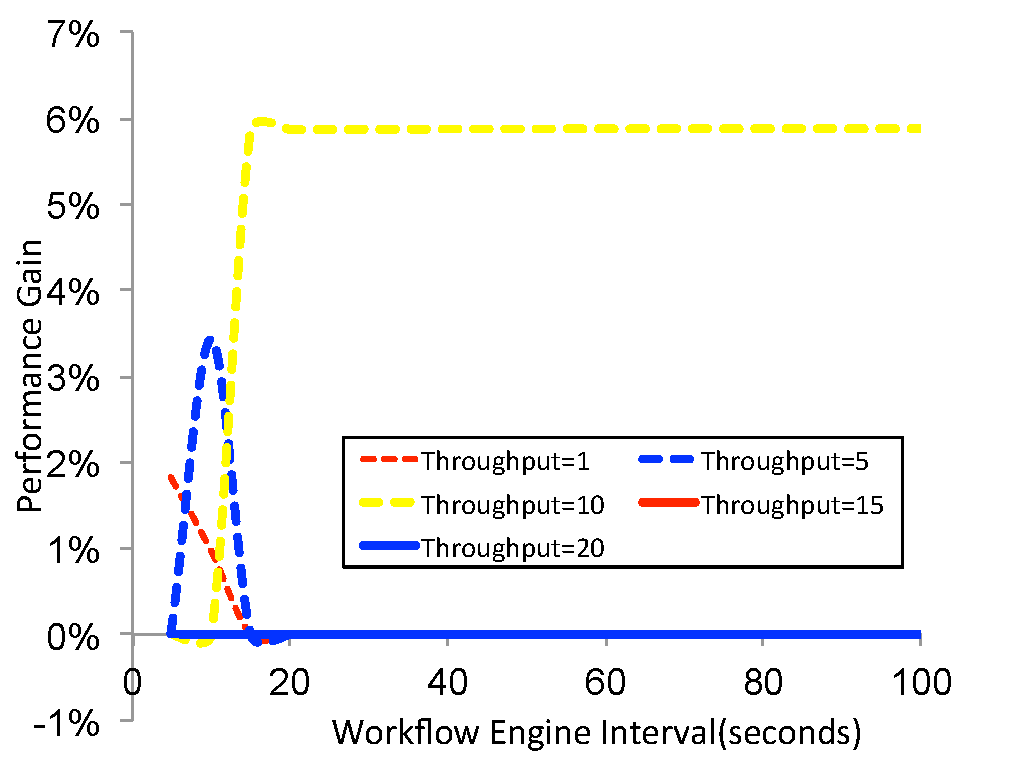
\includegraphics[width=0.9\linewidth]{figure/MAX-MIN-Montage.pdf}
  \captionof{figure}{Montage}
  \label{fig:MAX-MIN-Montage}
  \vspace{-10pt}
\end{figure}


Experiment 1: Fig.~\ref{fig:MAX-MIN-Broadband},~\ref{fig:MAX-MIN-CyberShake},~\ref{fig:MAX-MIN-Montage} show the  \emph{Performance Gain} of MAXMIN over MINMIN for the three workflows. We expected to see most  \emph{Performance Gain} $>0$ if MAXMIN is a overhead robust heuristic compared to MINMIN. However, except for the Montage workflow, the \emph{Performance Gain} is not significant for all of parameter settings, which concludes that MAXMIN is not globally overwhelming MINMIN in terms of overhead robustness. The reason we believe is that the  \emph{Performance Gain} in this comparison highly depends on the ratio of job runtime, workflow engine delay, number of resources and throughput of workflow engine. 

\begin{figure}[!htb]
\centering
 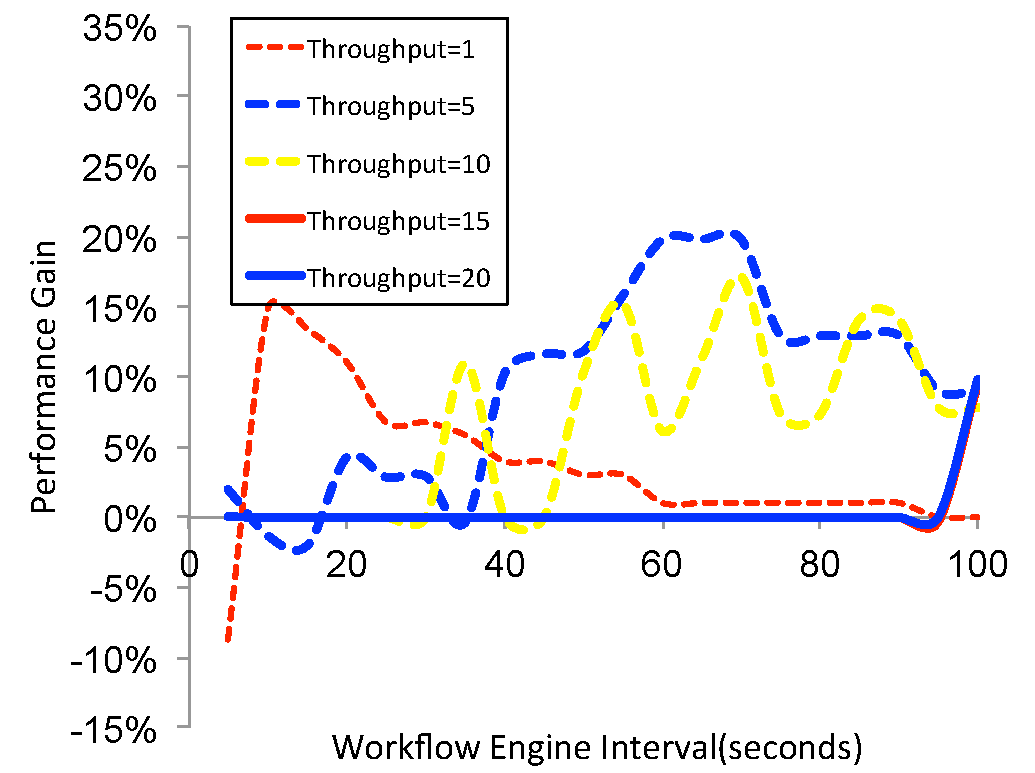
\includegraphics[width=0.9\linewidth]{figure/DFS-BFS-Broadband.pdf}
  \captionof{figure}{Broadband }
  \label{fig:DFS-BFS-Broadband}
  \vspace{-10pt}
\end{figure}

\begin{figure}[!htb]
\centering
 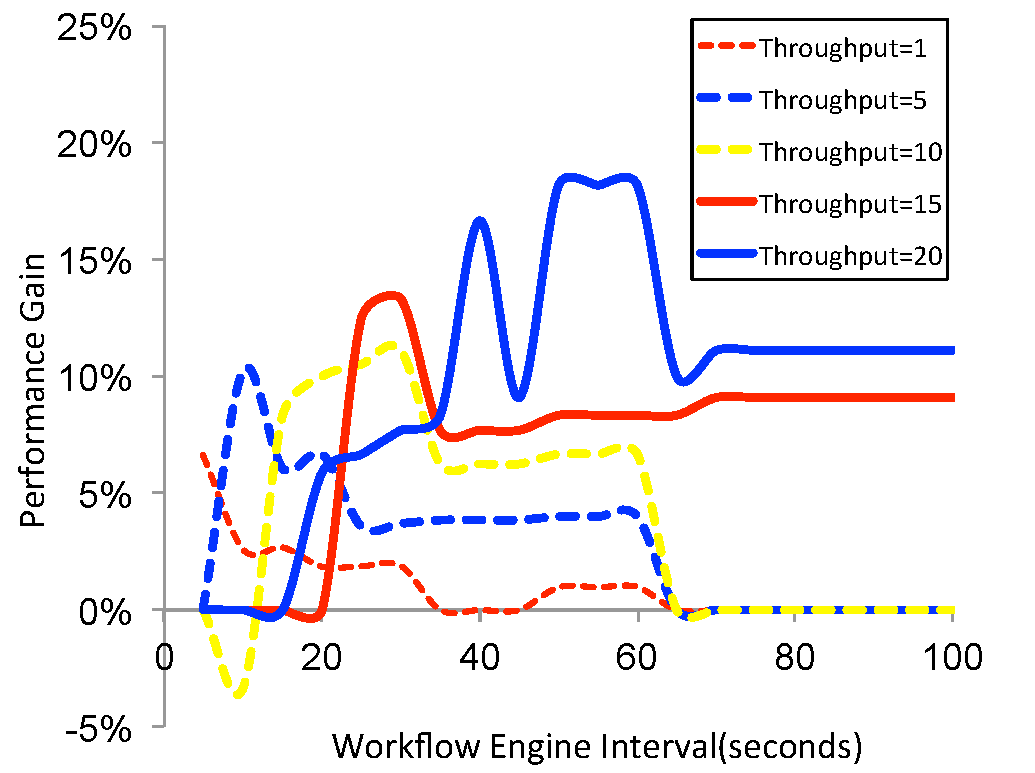
\includegraphics[width=0.9\linewidth]{figure/DFS-BFS-CyberShake.pdf}
  \captionof{figure}{CyberShake}
  \label{fig:DFS-BFS-CyberShake}
  \vspace{-10pt}
\end{figure}

\begin{figure}[!htb]
\centering
 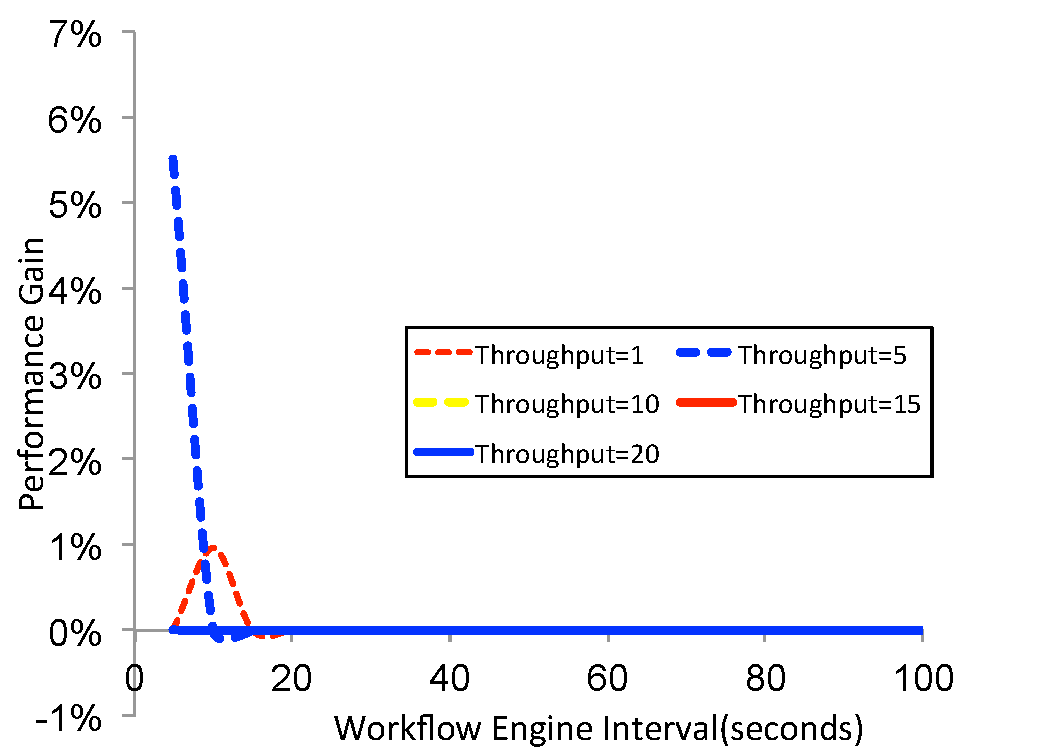
\includegraphics[width=0.9\linewidth]{figure/DFS-BFS-Montage.pdf}
  \captionof{figure}{Montage}
  \label{fig:DFS-BFS-Montage}
  \vspace{-10pt}
\end{figure}


Experiment 2: Fig.~\ref{fig:DFS-BFS-Broadband},~\ref{fig:DFS-BFS-CyberShake},~\ref{fig:DFS-BFS-Montage} show the \emph{Performance Gain} of BFS over DFS for the three workflows. We observe that most  \emph{Performance Gain} $>0$ and thus BFS performs better than DFS in terms of overhead robustness. What is more, Fig~\ref{fig:DFS-BFS-CyberShake} shows with the increase of average throughput, the \emph{Performance Gain} is more significant. We can also see that when the average throughput is high, the \emph{Performance Gain} increases with the average interval of workflow engine. This suggests us in a real environment with a large overhead, we should use BFS instead of DFS. 


\begin{figure}[!htb]
\centering
 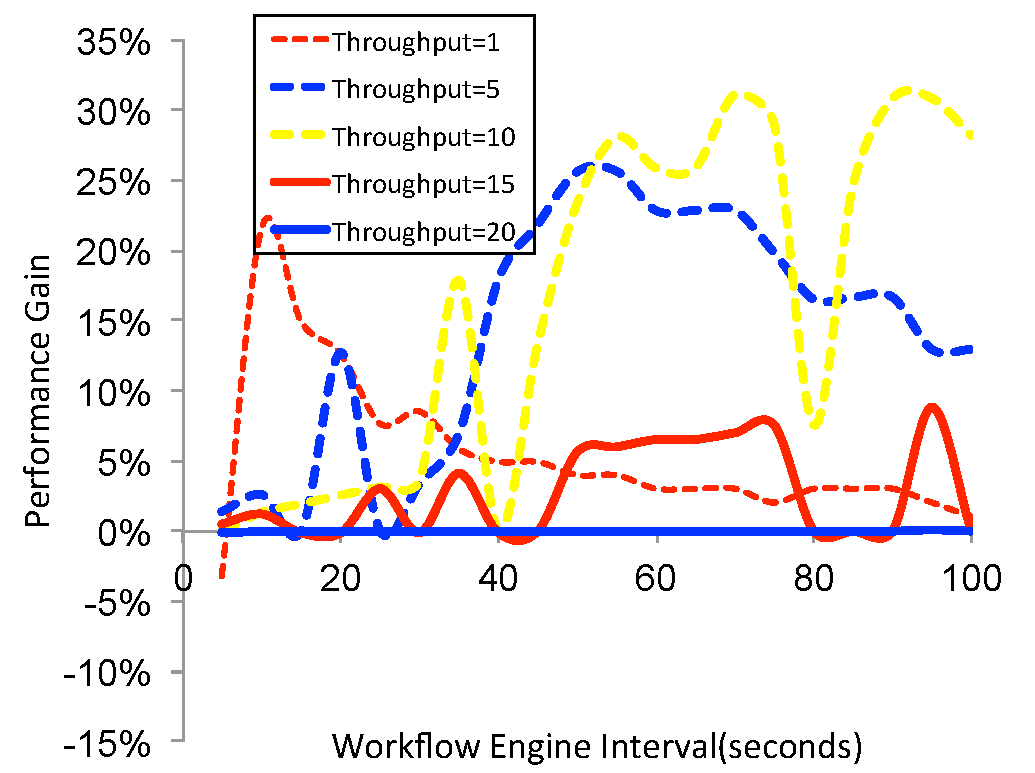
\includegraphics[width=0.9\linewidth]{figure/UFFS-FFS-Broadband.pdf}
  \captionof{figure}{Broadband }
  \label{fig:UFFS-FFS-Broadband}
  \vspace{-10pt}
\end{figure}

\begin{figure}[!htb]
\centering
 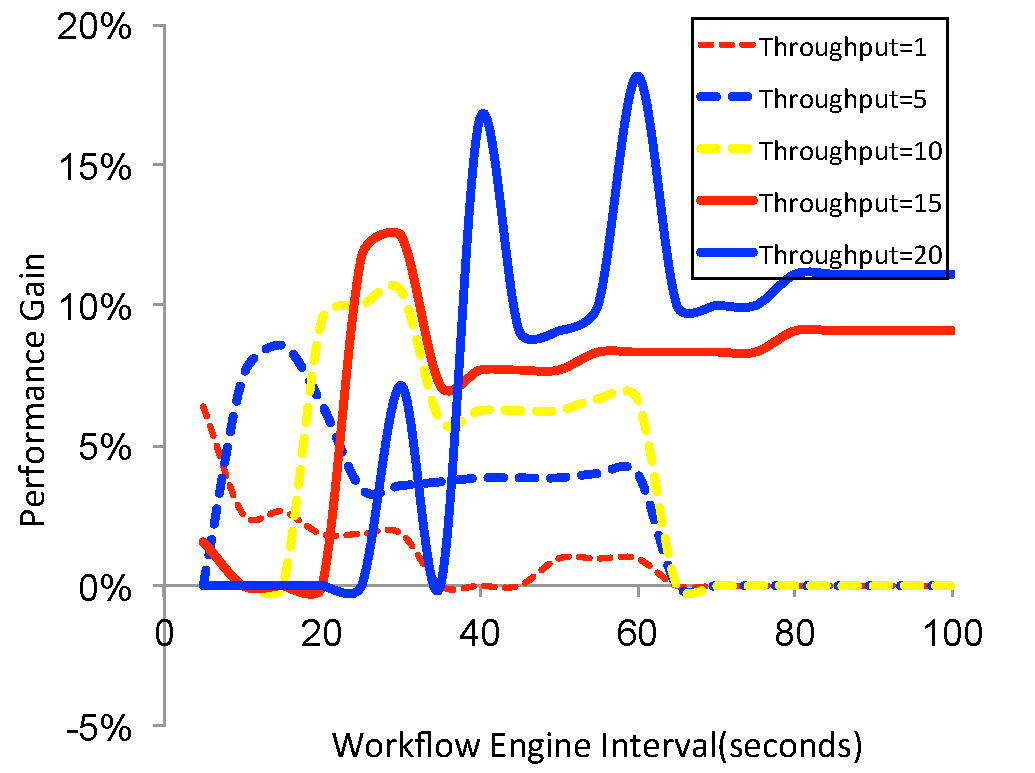
\includegraphics[width=0.9\linewidth]{figure/UFFS-FFS-CyberShake.pdf}
  \captionof{figure}{CyberShake}
  \label{fig:UFFS-FFS-CyberShake}
  \vspace{-10pt}
\end{figure}

\begin{figure}[!htb]
\centering
 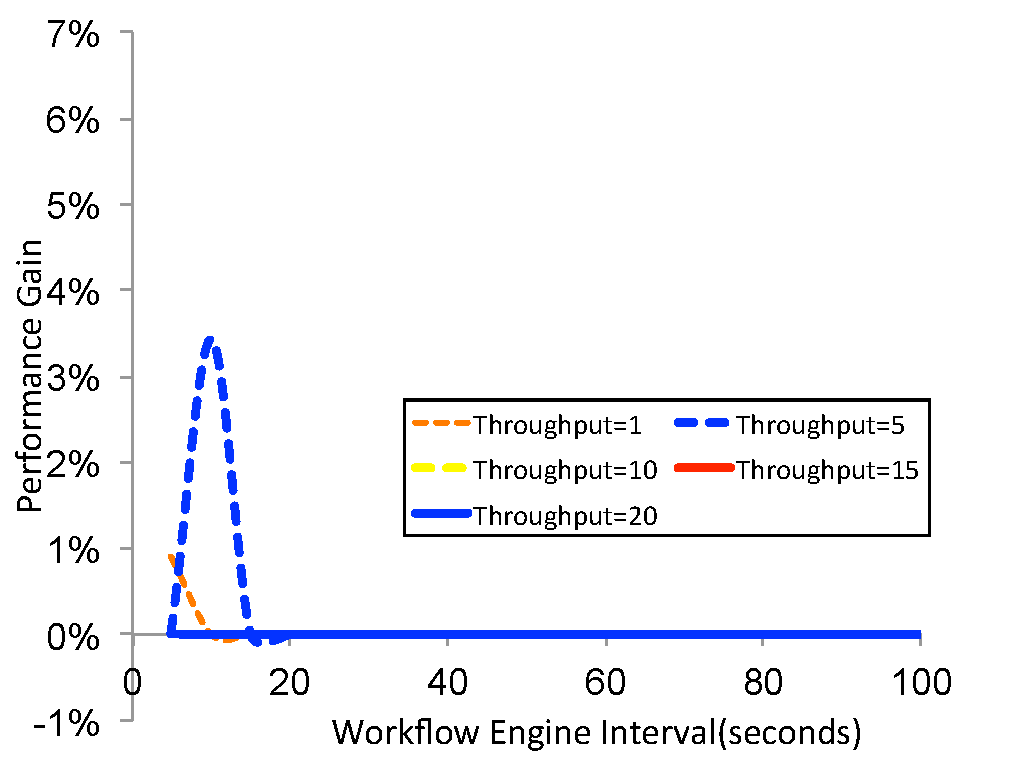
\includegraphics[width=0.9\linewidth]{figure/UFFS-FFS-Montage.pdf}
  \captionof{figure}{Montage}
  \label{fig:UFFS-FFS-Montage}
  \vspace{-10pt}
\end{figure}



Experiment 3: Fig.~\ref{fig:UFFS-FFS-Broadband},~\ref{fig:UFFS-FFS-CyberShake},~\ref{fig:UFFS-FFS-Montage} show the \emph{Performance Gain} of FFS over UFFS for the three workflows. We observe that most  \emph{Performance Gain} $>0$ and thus FFS performs better than UFFS in terms of overhead robustness, which is similar to Experiment 2. Comparing Fig.~\ref{fig:DFS-BFS-Broadband} and Fig.~\ref{fig:UFFS-FFS-Broadband} we can see the \emph{Performance Gain} of FFS over UFFS is more significant (30\%) than that of BFS over DFS (20\%).  
\begin{figure}[!htb]
\centering
 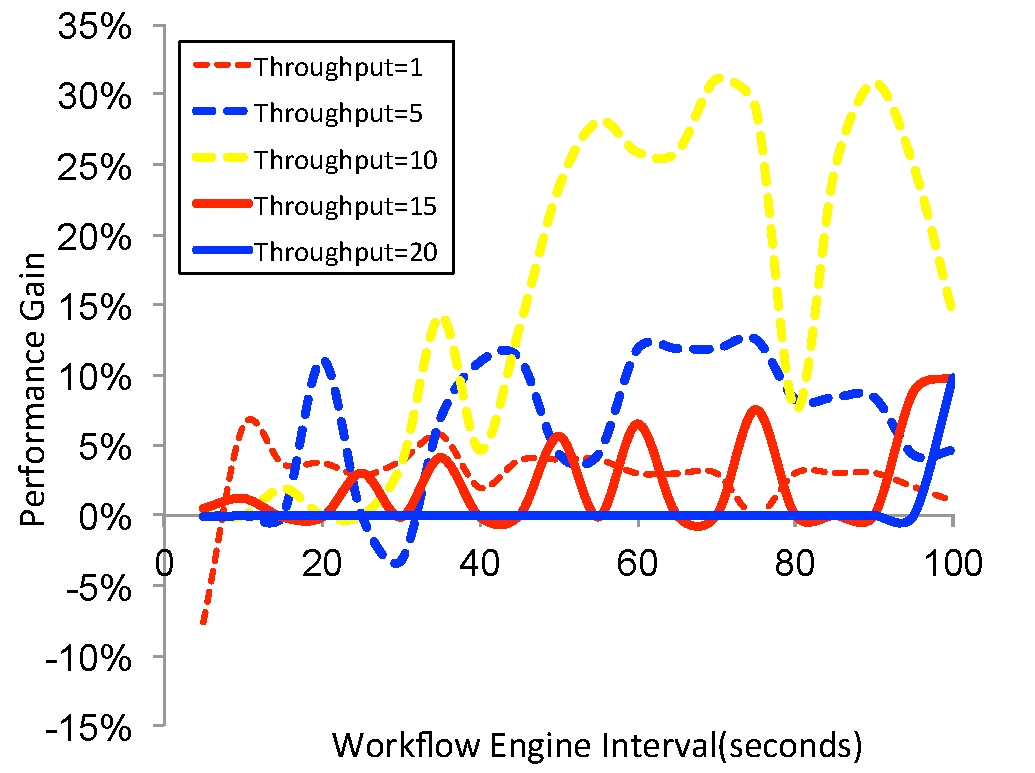
\includegraphics[width=0.9\linewidth]{figure/UIFS-IFS-Broadband.pdf}
  \captionof{figure}{Broadband }
  \label{fig:UIFS-IFS-Broadband}
  \vspace{-10pt}
\end{figure}

\begin{figure}[!htb]
\centering
 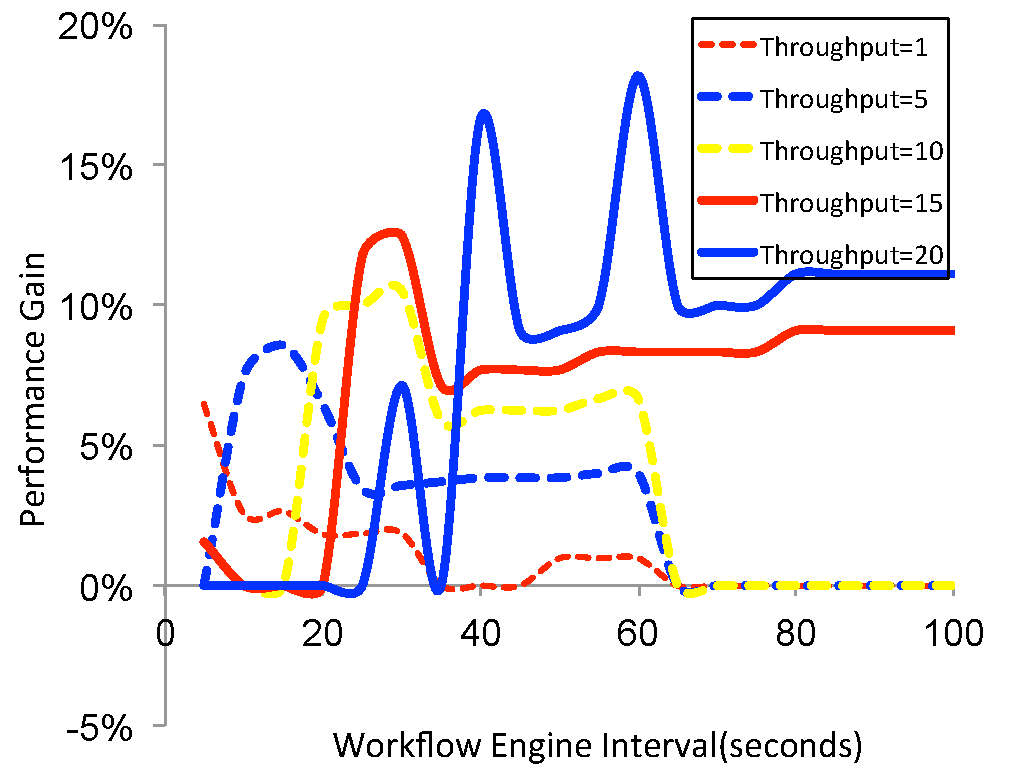
\includegraphics[width=0.9\linewidth]{figure/UIFS-IFS-CyberShake.pdf}
  \captionof{figure}{CyberShake}
  \label{fig:UIFS-IFS-CyberShake}
  \vspace{-10pt}
\end{figure}

\begin{figure}[!htb]
\centering
 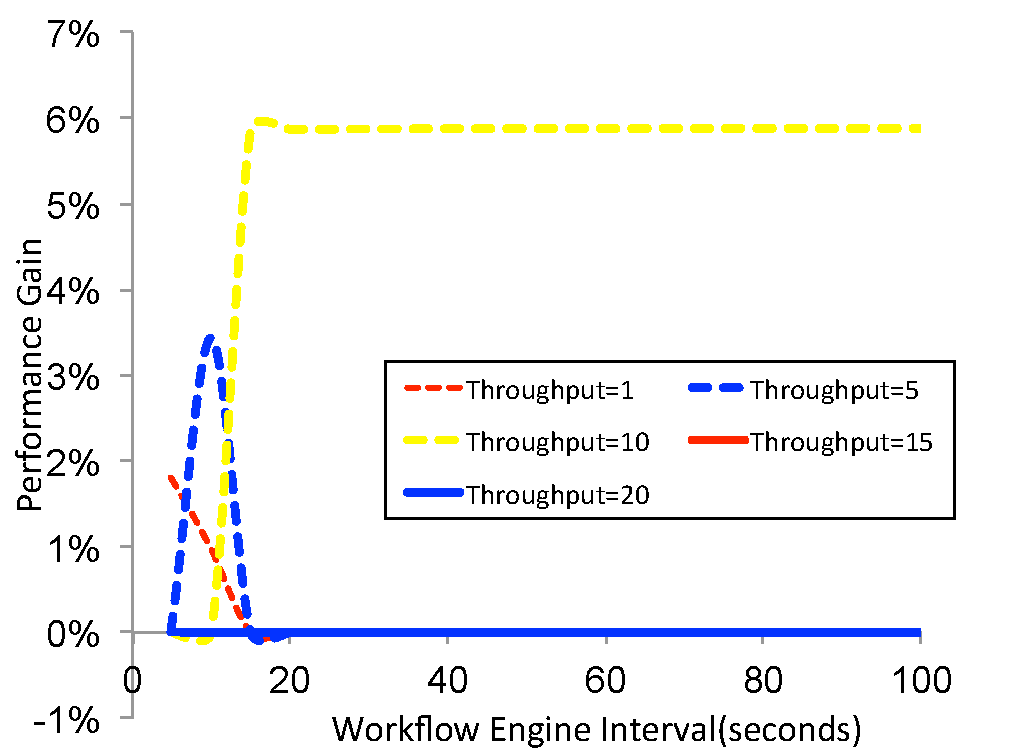
\includegraphics[width=0.9\linewidth]{figure/UIFS-IFS-Montage.pdf}
  \captionof{figure}{Montage}
  \label{fig:UIFS-IFS-Montage}
  \vspace{-10pt}
\end{figure}
Experiment 4: Fig.~\ref{fig:UIFS-IFS-Broadband},~\ref{fig:UIFS-IFS-CyberShake},~\ref{fig:UIFS-IFS-Montage} show the \emph{Performance Gain} of IFS over UIFS for the three workflows. We observe that most  \emph{Performance Gain} $>0$ and thus IFS performs better than UIFS in terms of overhead robustness, which is similar to Experiment 3. The reason is that for these workflows, IF based heuristics can produce similar schedule as the heuristics based on the number of children. Most of the workflows used in this paper is not irregular enough and thus we are not able to show the difference of IF based heuristics and the heuristics based on the number of children. 



\section{Conclusion, Discussion and Future Work}

In this work, we introduced a series of quantitative and structural metrics in revealing workflow structure information and we further applied them to three usage scenario to show their influence with traced based analysis and simulations. The experiments show that these metrics can significantly improve the performance of task clustering strategies and task scheduling strategies.   

In our work, we have shown that these metrics have strong connection with the performance of different optimization methods. However, not all of them perform well under all of the circumstances. Also, the origin of these metrics are heavily depending on human intuition. Still, there is a lack of understanding of whether we can have more and better metrics in revealing how workflow structures interact with different optimization methods. As an initial effort, we will continue to use pattern discovery techniques to collect as many metrics as possible and performance experiments on them. 

With enough metrics, one important step we are going to take is to aggregate multiple metrics and use machine learning techniques to reveal their correlation. However, combining the metrics we have proposed above is challenging. First, these metrics are quantitative and can be measured, however, on their own they are hard to compare against each other and determine whether one metric is more significant than others. Second,  having multiple metrics together increase the complexity and this is against our initial goal, which is reduce the complexity in analyzing workflows. A more sophisticated alternative, however, is to conduct a statistical analysis based on Principal Component Analysis (PCA). This method determines in a more precise way the existing correlation between the collected metrics and their impact on workflow performance.

%A more sophisticated alternative, however, is to conduct a statistical analysis based on Principal Component Analysis (PCA). This method determines in a more precise way the existing correlation between the collected metrics and their impact on resilience. However, undertaking an automated analysis using PCA requires prior experimental data to be available. For this reason, in or- der to better enable a comparison, the aggregation of all the metrics into a single value is proposed in this section. Aggregations of multiple variables are used in many well- known disciplines such as statistical or economic measure- ment. However, combining the metrics we have proposed above provides three main challenges. First, the metrics are quantitative and can be measured, however on their own they are hard to compare against each other and to deter- mine whether one metric is more significant than another. Second, having multiple metrics makes any comparison difficult. Third, resilience increases in direct proportion to some metrics, whereas it reduces with respect to others. Identify- ing to what degree each measured metric impacts resilience (directly or inversely) must also be qualified through previously recorded experimental data or by an expert.

%% References with bibTeX database:

\bibliographystyle{elsarticle-num}
\bibliography{biblio}

%% Authors are advised to submit their bibtex database files. They are
%% requested to list a bibtex style file in the manuscript if they do
%% not want to use elsarticle-num.bst.

%% References without bibTeX database:

% \begin{thebibliography}{00}

%% \bibitem must have the following form:
%%   \bibitem{key}...
%%

% \bibitem{}

% \end{thebibliography}


\end{document}

%%
%% End of file `elsarticle-template-num.tex'.
